\label{chp:bgm}
%\lipsum[101-120]
\section{The Building Game as a Mathematical Framework for Self-assembly}

The Building Game was first introduced by Wales~\cite{Wales1987} as a model for the formation of close-boranes. Zlotnick subsequently altered the Building Game and used it as a model for the assembly of polyhedral viral capsids~\cite{Zlotnick1994}. In the model, a capsid is idealized as a polyhedron with each face treated as a subunit. Assembly proceeds from a singe face with a second face attached to the first along an edge. At each subsequent step of the process, an additional face is added along an edge of one of the already added faces. The process ends when all of the faces have been added resulting in a completed polyhedron.

A useful way to think about the Building Game is as a sequential coloring process. Given a polyhedron with each face painted white, choose a face and paint it black. At each subsequent step, choose a white face that is adjacent to a black face and paint it black. Repeat until all faces are black. Here the black faces represent a face being present at a given step of the assembly process.

%--Comparison with approaches in artificial life paper


\section{Formal Definition}
We formalize the Building Game in terms of the group action of the polyhedron's rotation group $G$ acting on subsets of $F$, the polyhedron's face set. Using the polyhedron's dual graph $\PolyGraph\left(F, E\right)$ whose nodes are the faces $F$ of the polyhedron and connections $E$ correspond to the pairs of faces sharing an edge we can define the mathematical structures that comprise different Building Game configurations.


%If we are interested in the Building Game of a polyhedron, we represent the its combinatorial structure by a graph $\PolyGraph = \left(F, E\right)$ whose nodes are the faces $F$ of the polyhedron and connections $E$ correspond to the pairs of faces sharing an edge. In this way, $\PolyGraph$ can be viewed as the polyhedral graph of \poly's dual polyhedron. 

\begin{mydef}
  A Building Game \textbf{state} $x \subset F$ is a non-empty subset of the faces $F$ of a polyhedron such that the sub-graph of $\PolyGraph$ restricted to $x$, $\PolyGraph|_x$, is a single connected component. As a result, every state can be formed through the Building Game attachment process.  
\end{mydef} 

Schlegel diagrams are two dimensional projections of the three dimensional polyhedron~\cite{Sommerville1929}. By coloring different subsets of faces, it is often useful to depict Building Game states with Schlegel diagrams.  Figure~\ref{fig:TetraStates} uses Schlegel diagrams to depicts all of the states of the tetrahedron. Since every face of the tetrahedron is adjacent to every other face, any non-empty subset of faces is a Building Game state. Thus, there are ${4 \choose k}$ tetrahedron states that have $k$ faces and $2^4 - 1 = 15$ states in total. 
\begin{figure}[ht]
\centering
  %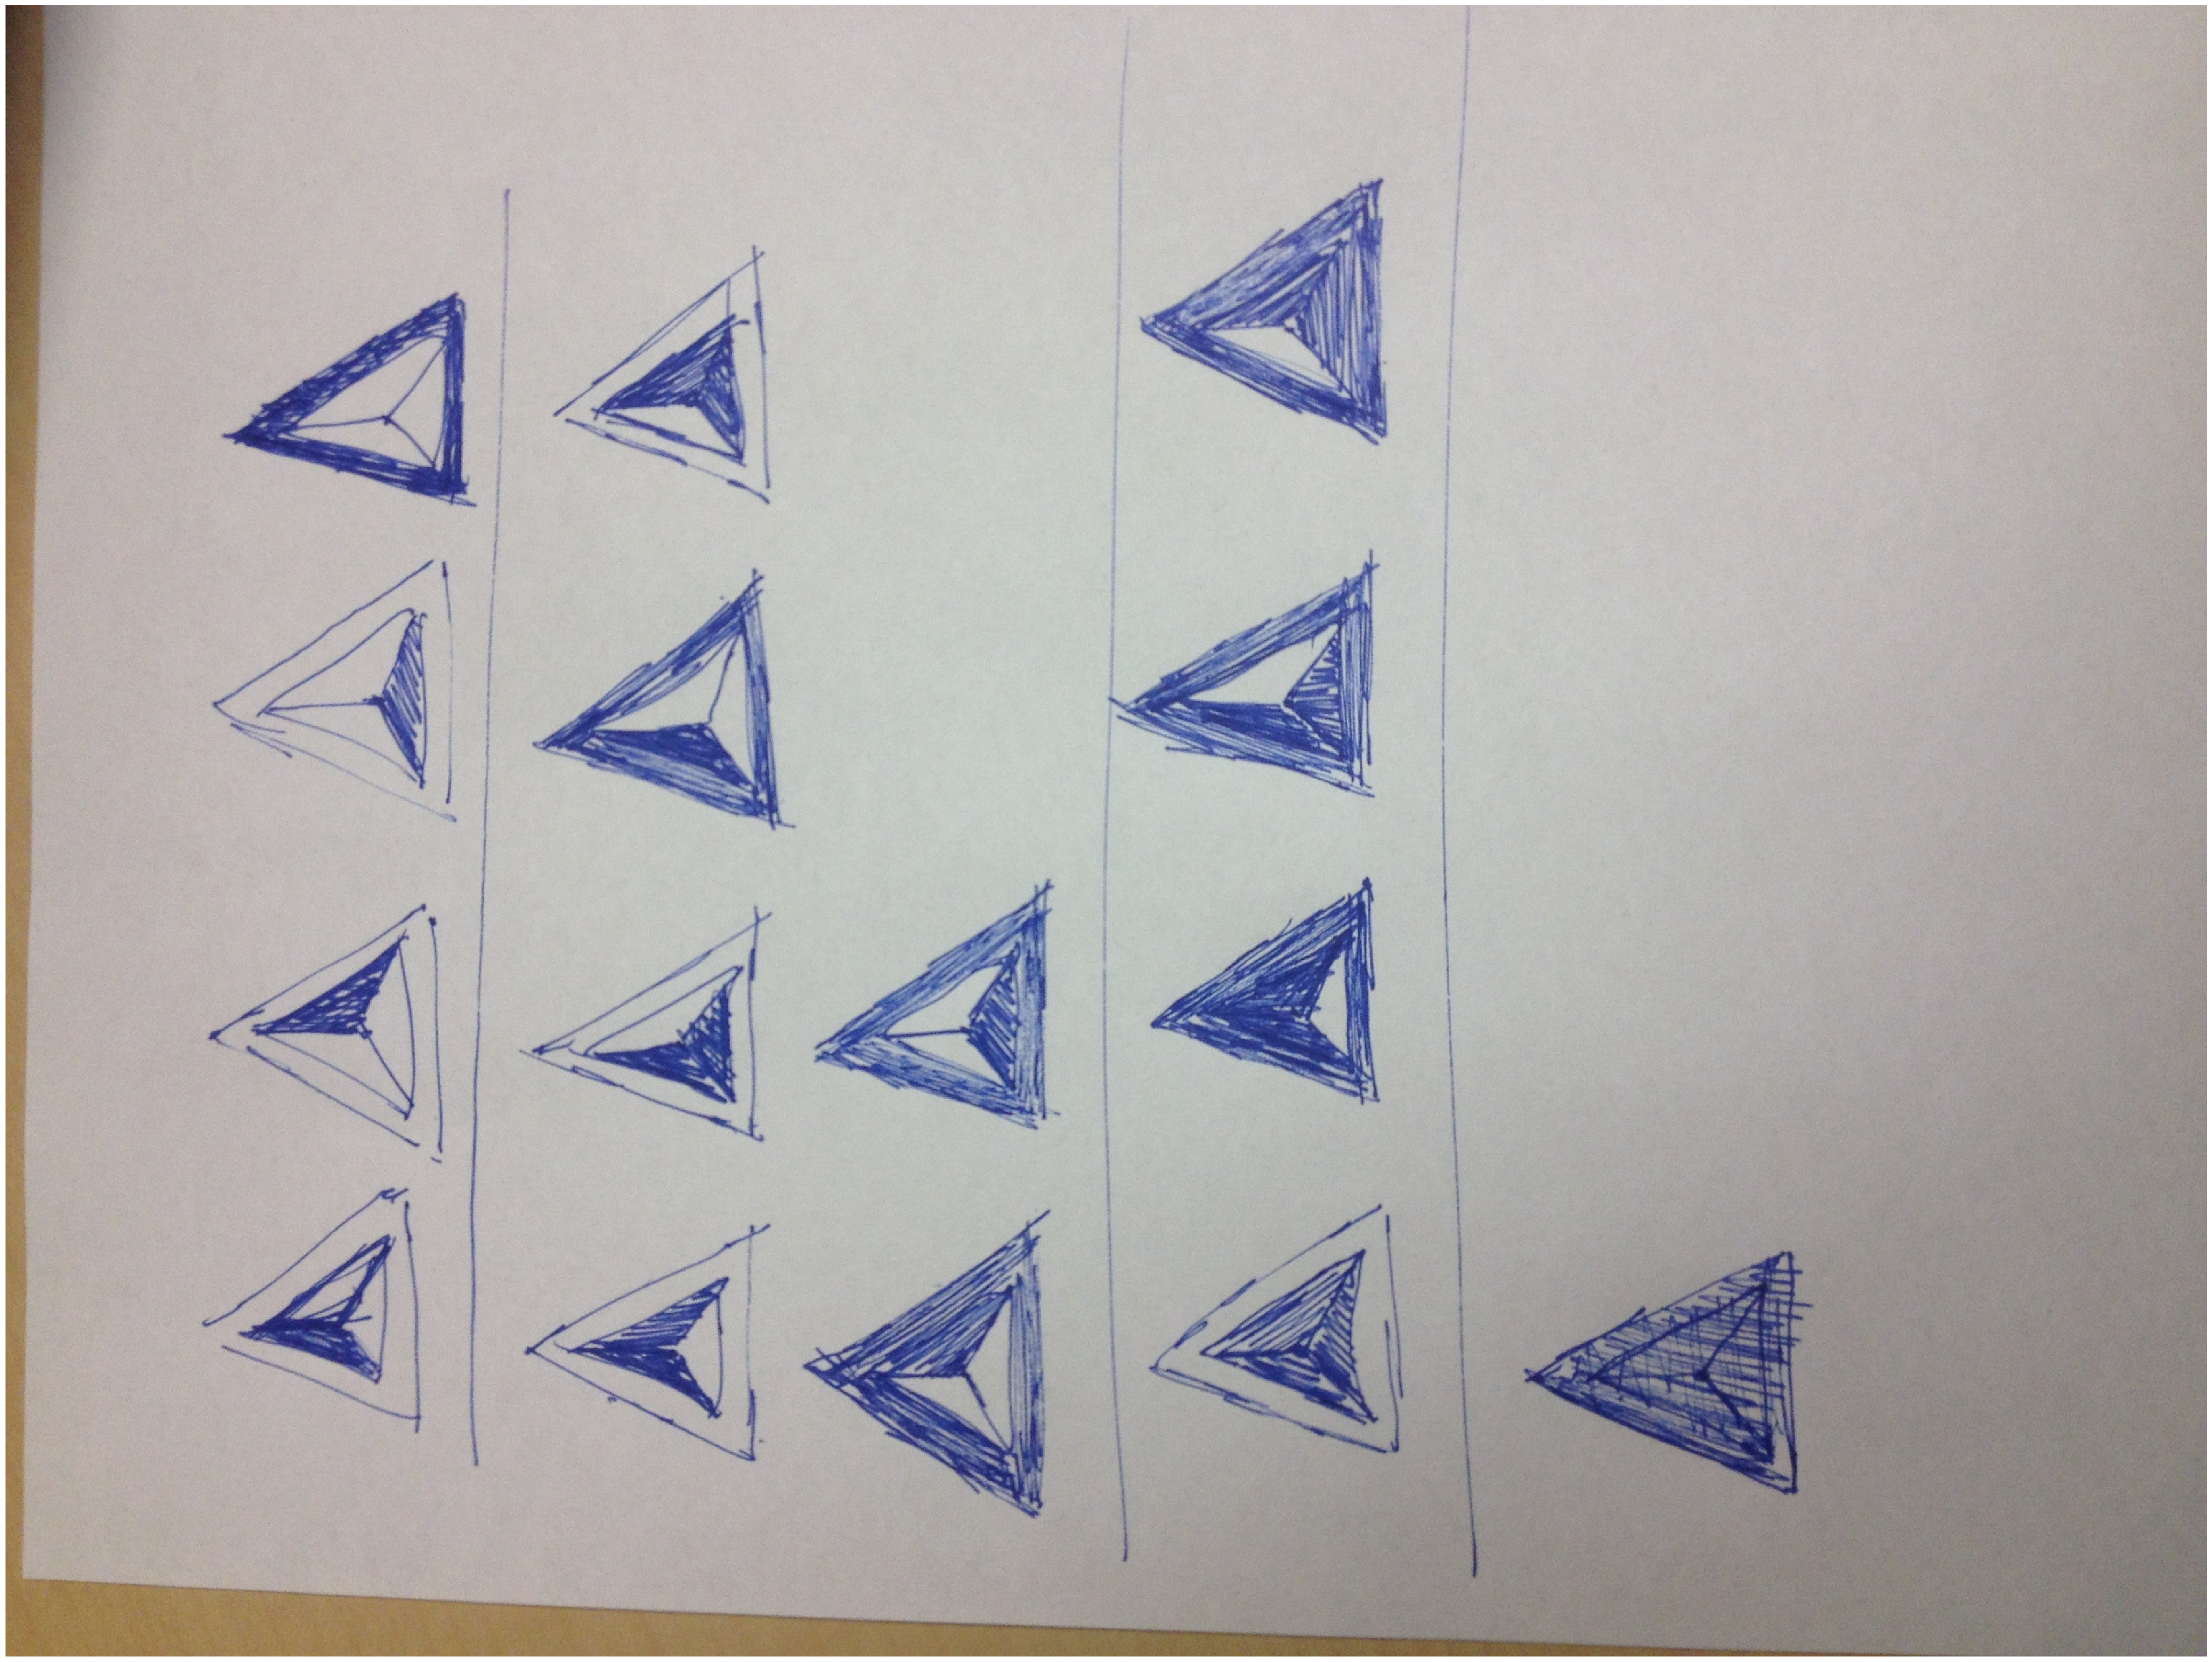
\includegraphics[scale=0.1, angle=0]{tetrahedron_states.eps}
  %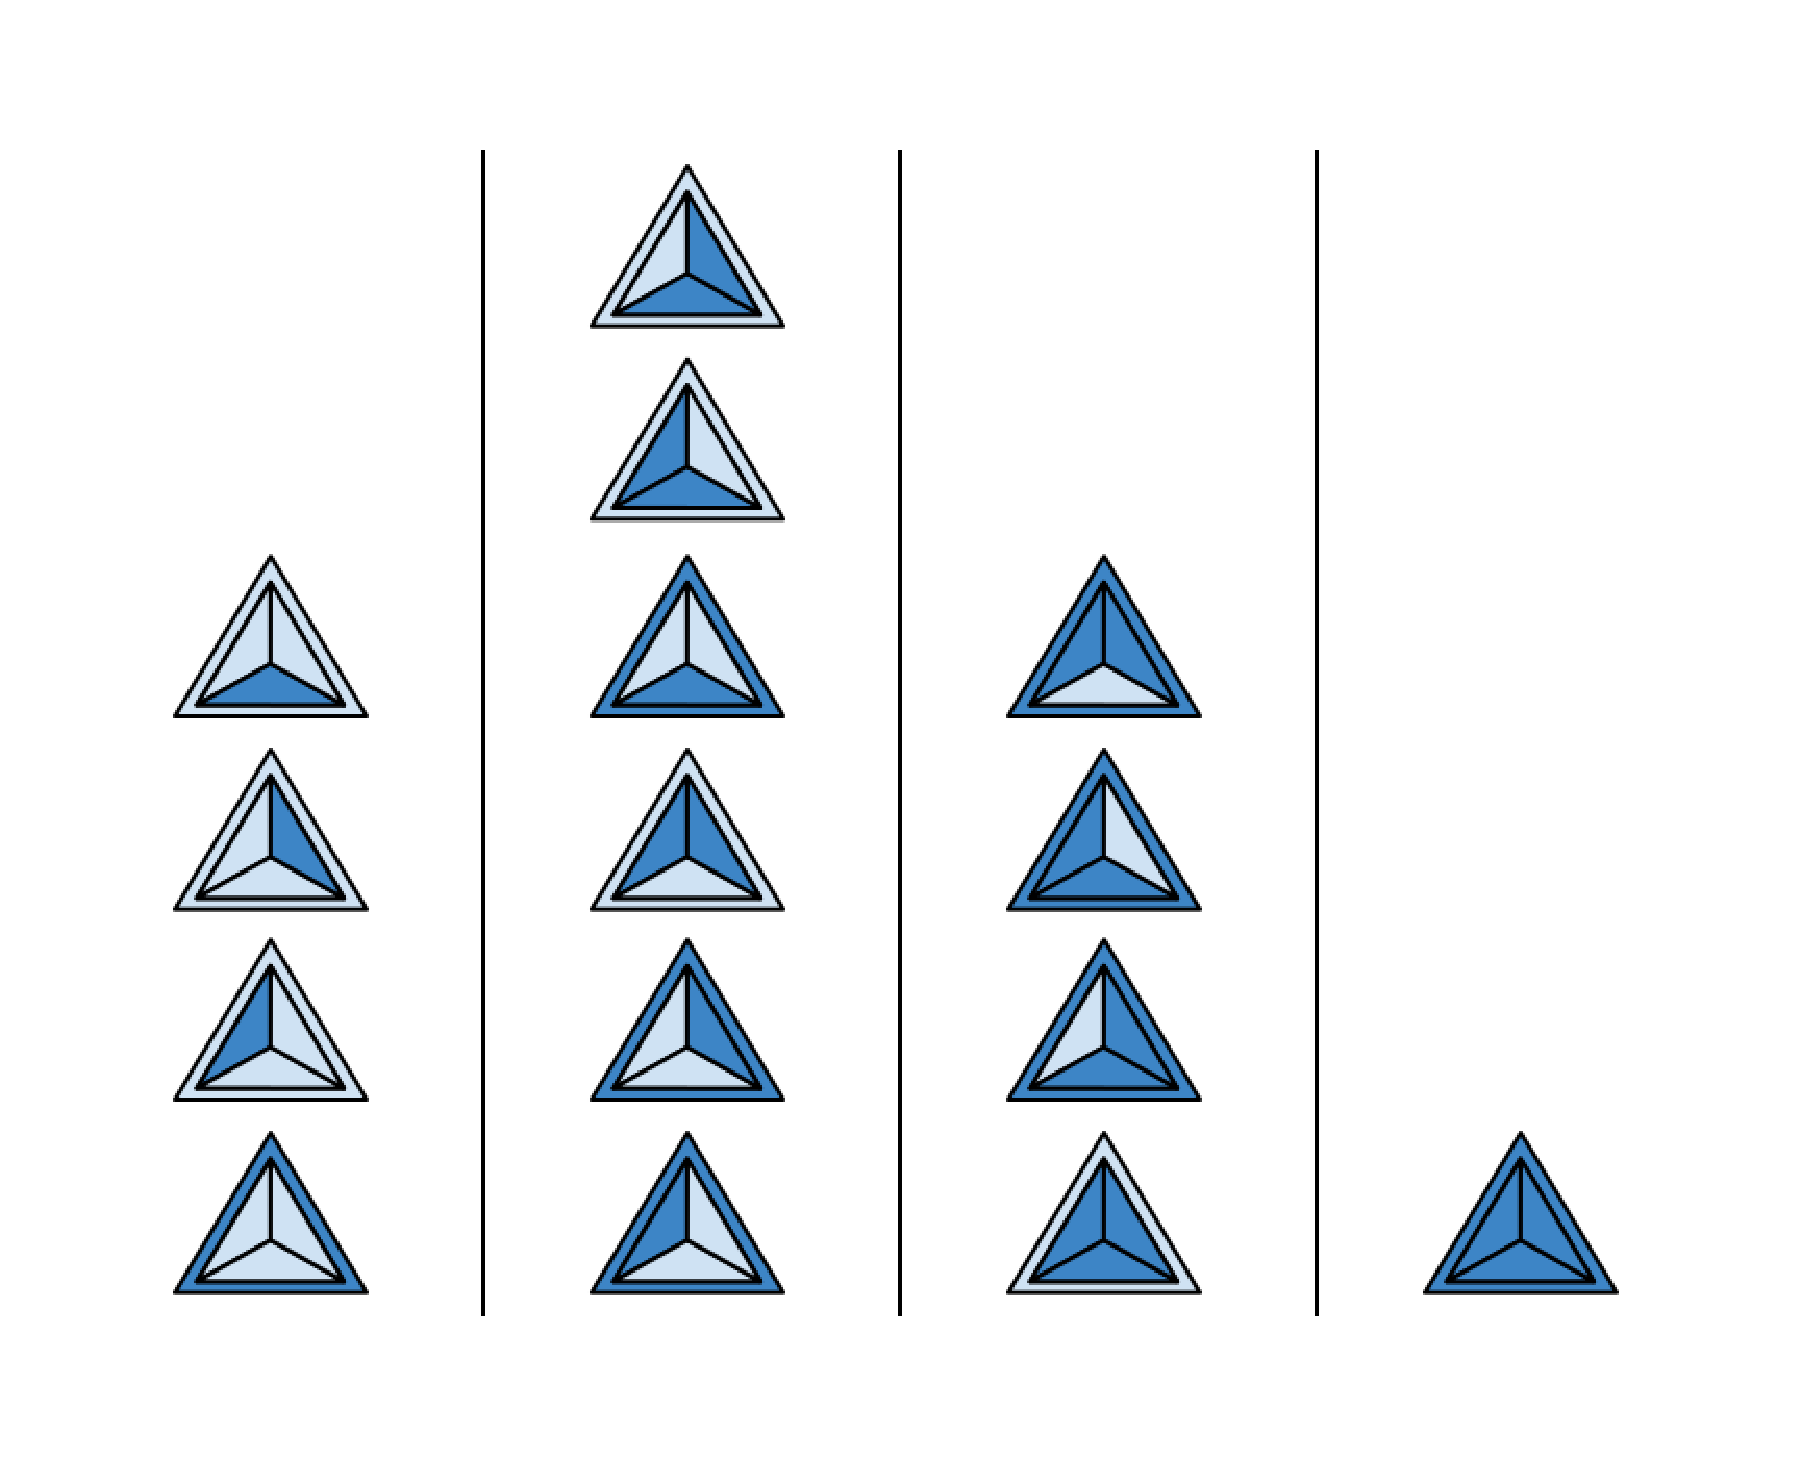
\includegraphics[scale=0.5, angle=0]{tetrahedron_states_2.eps}
  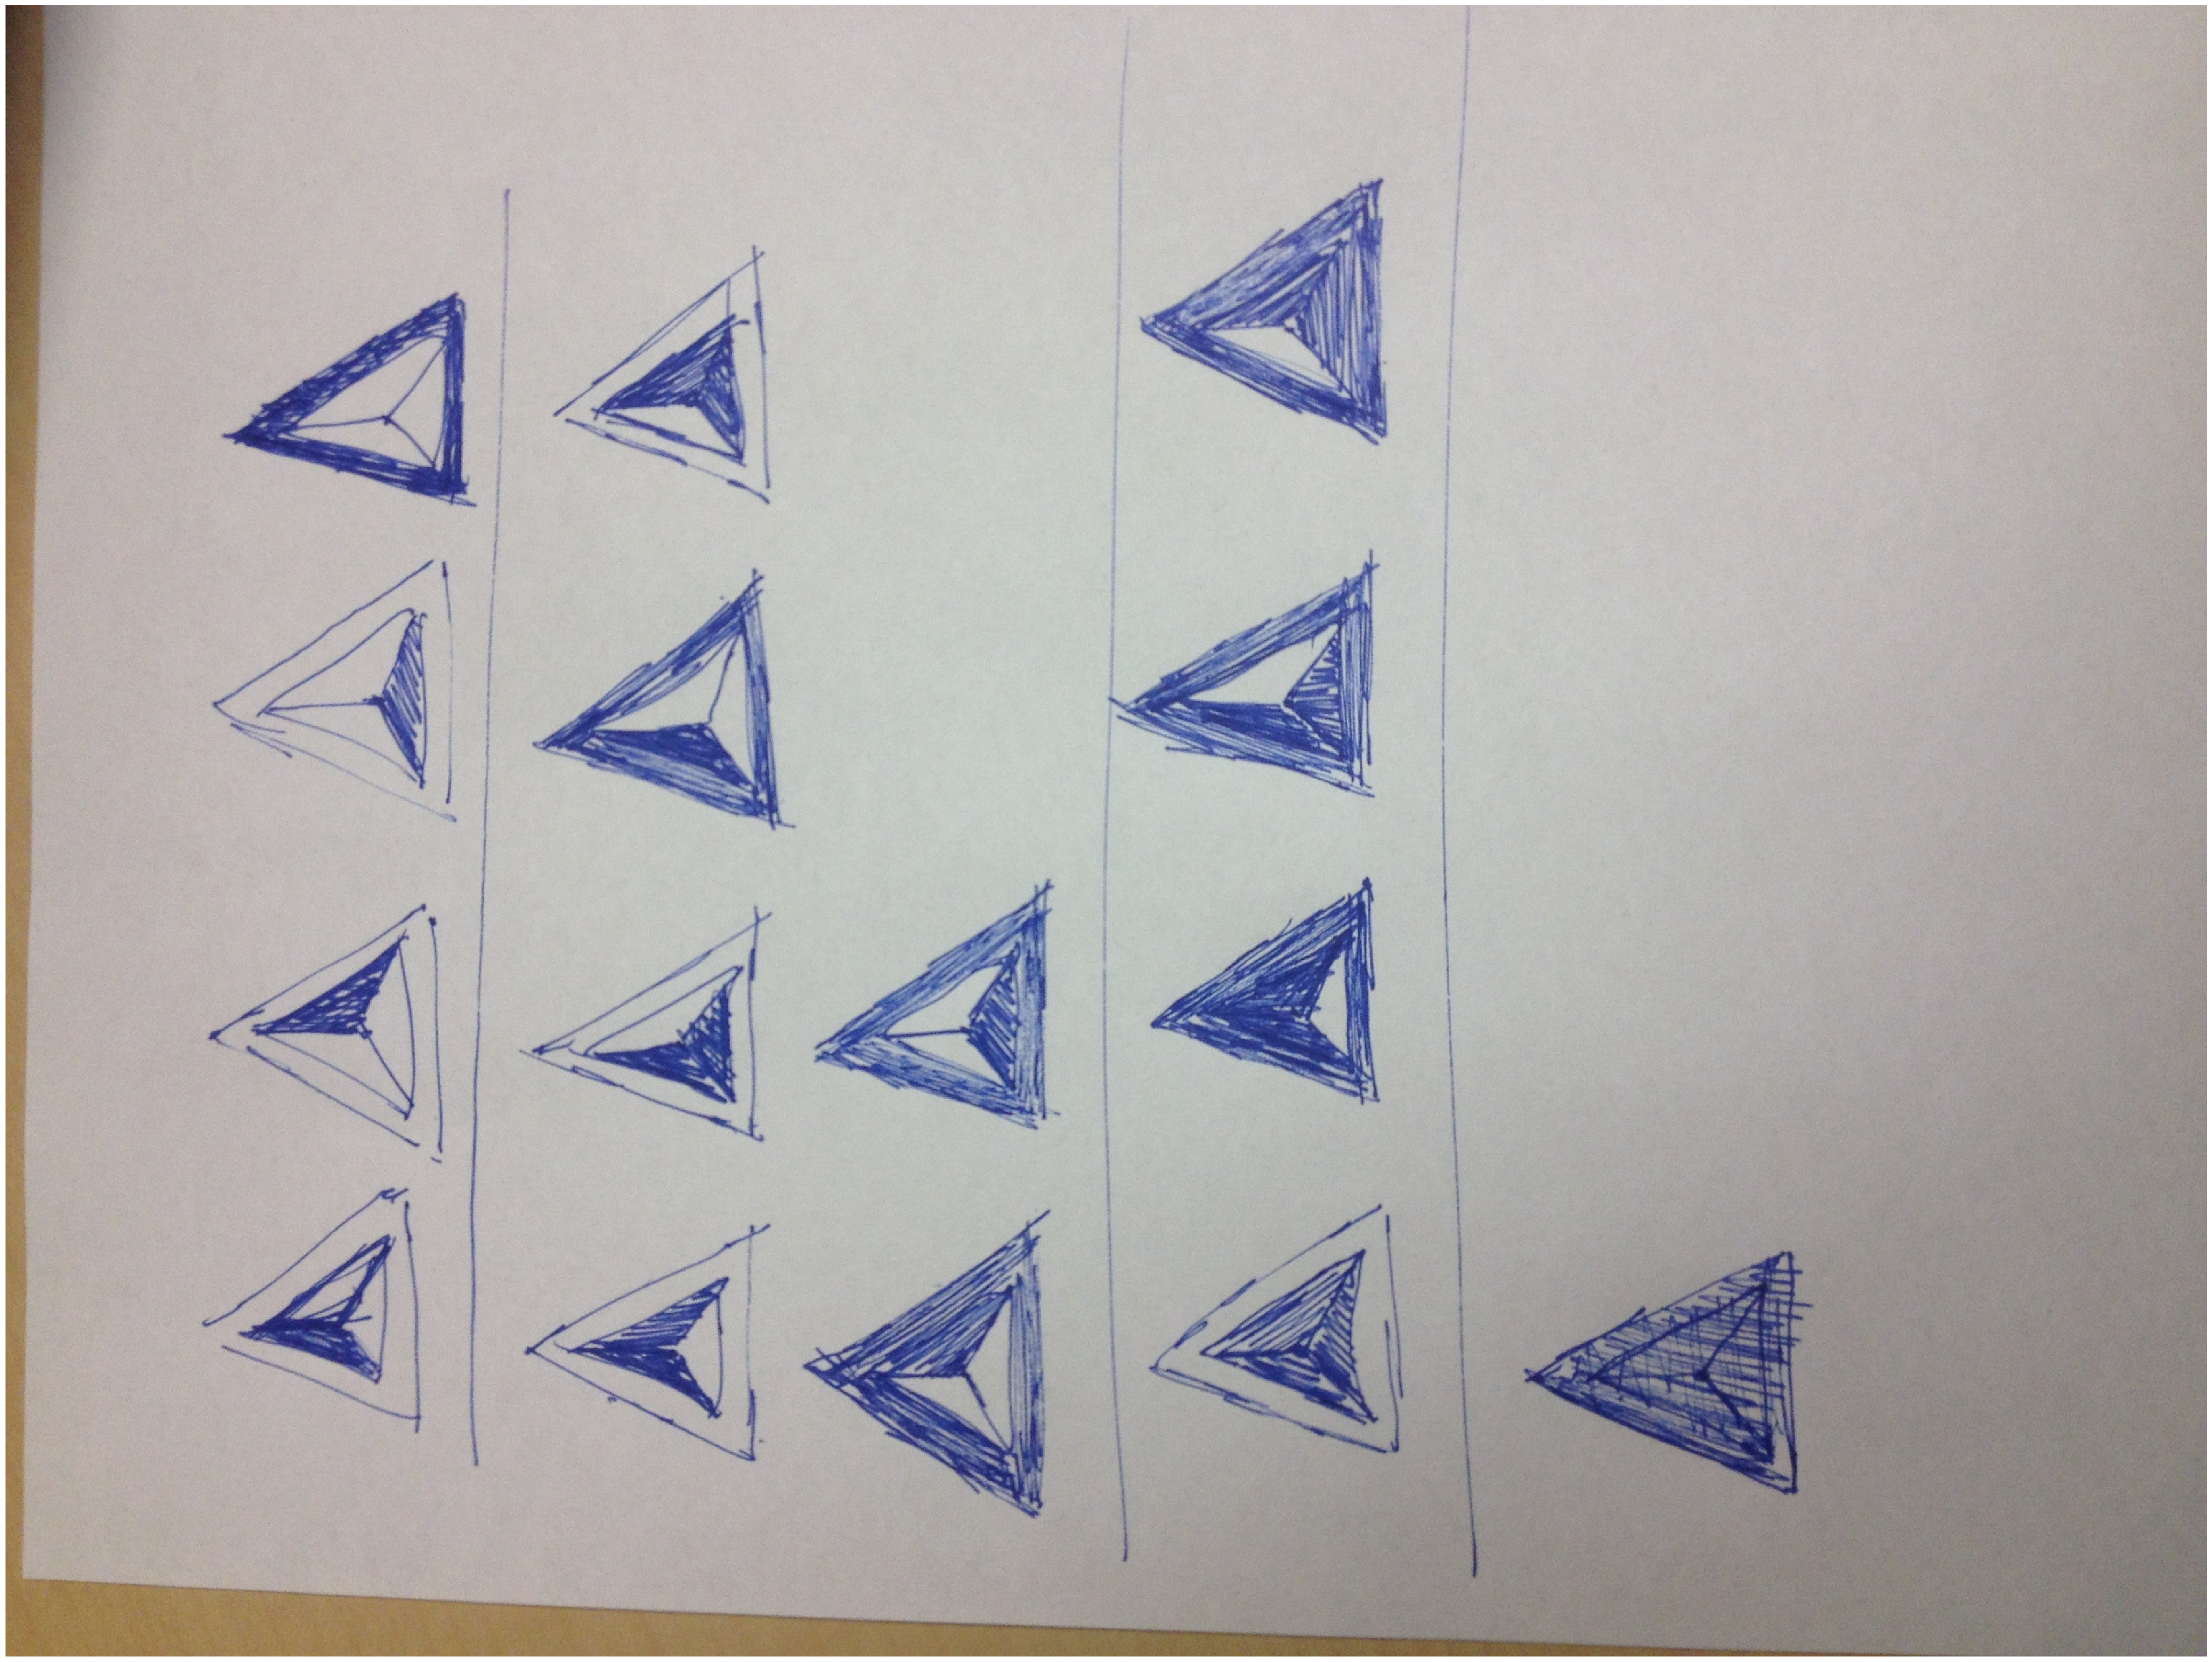
\includegraphics[scale=0.04, angle=0]{tetrahedron_states.eps}
\caption{The Building Game states of the tetrahedron.}
\label{fig:TetraStates}
\end{figure}
As pictured in figure~\ref{fig:OctaStates}, some subsets of faces are not states. For instance, the subset of octahedron faces with only two faces that are not adjacent is not a state. Similarly, the subset of two faces meeting only at a vertex is not a state as they are not connected through edge adjacency in the graph $\PolyGraph$. However, when more faces are added to connect these faces in $\PolyGraph$ the subset is indeed a state.

\begin{figure}[ht]
        \centering
  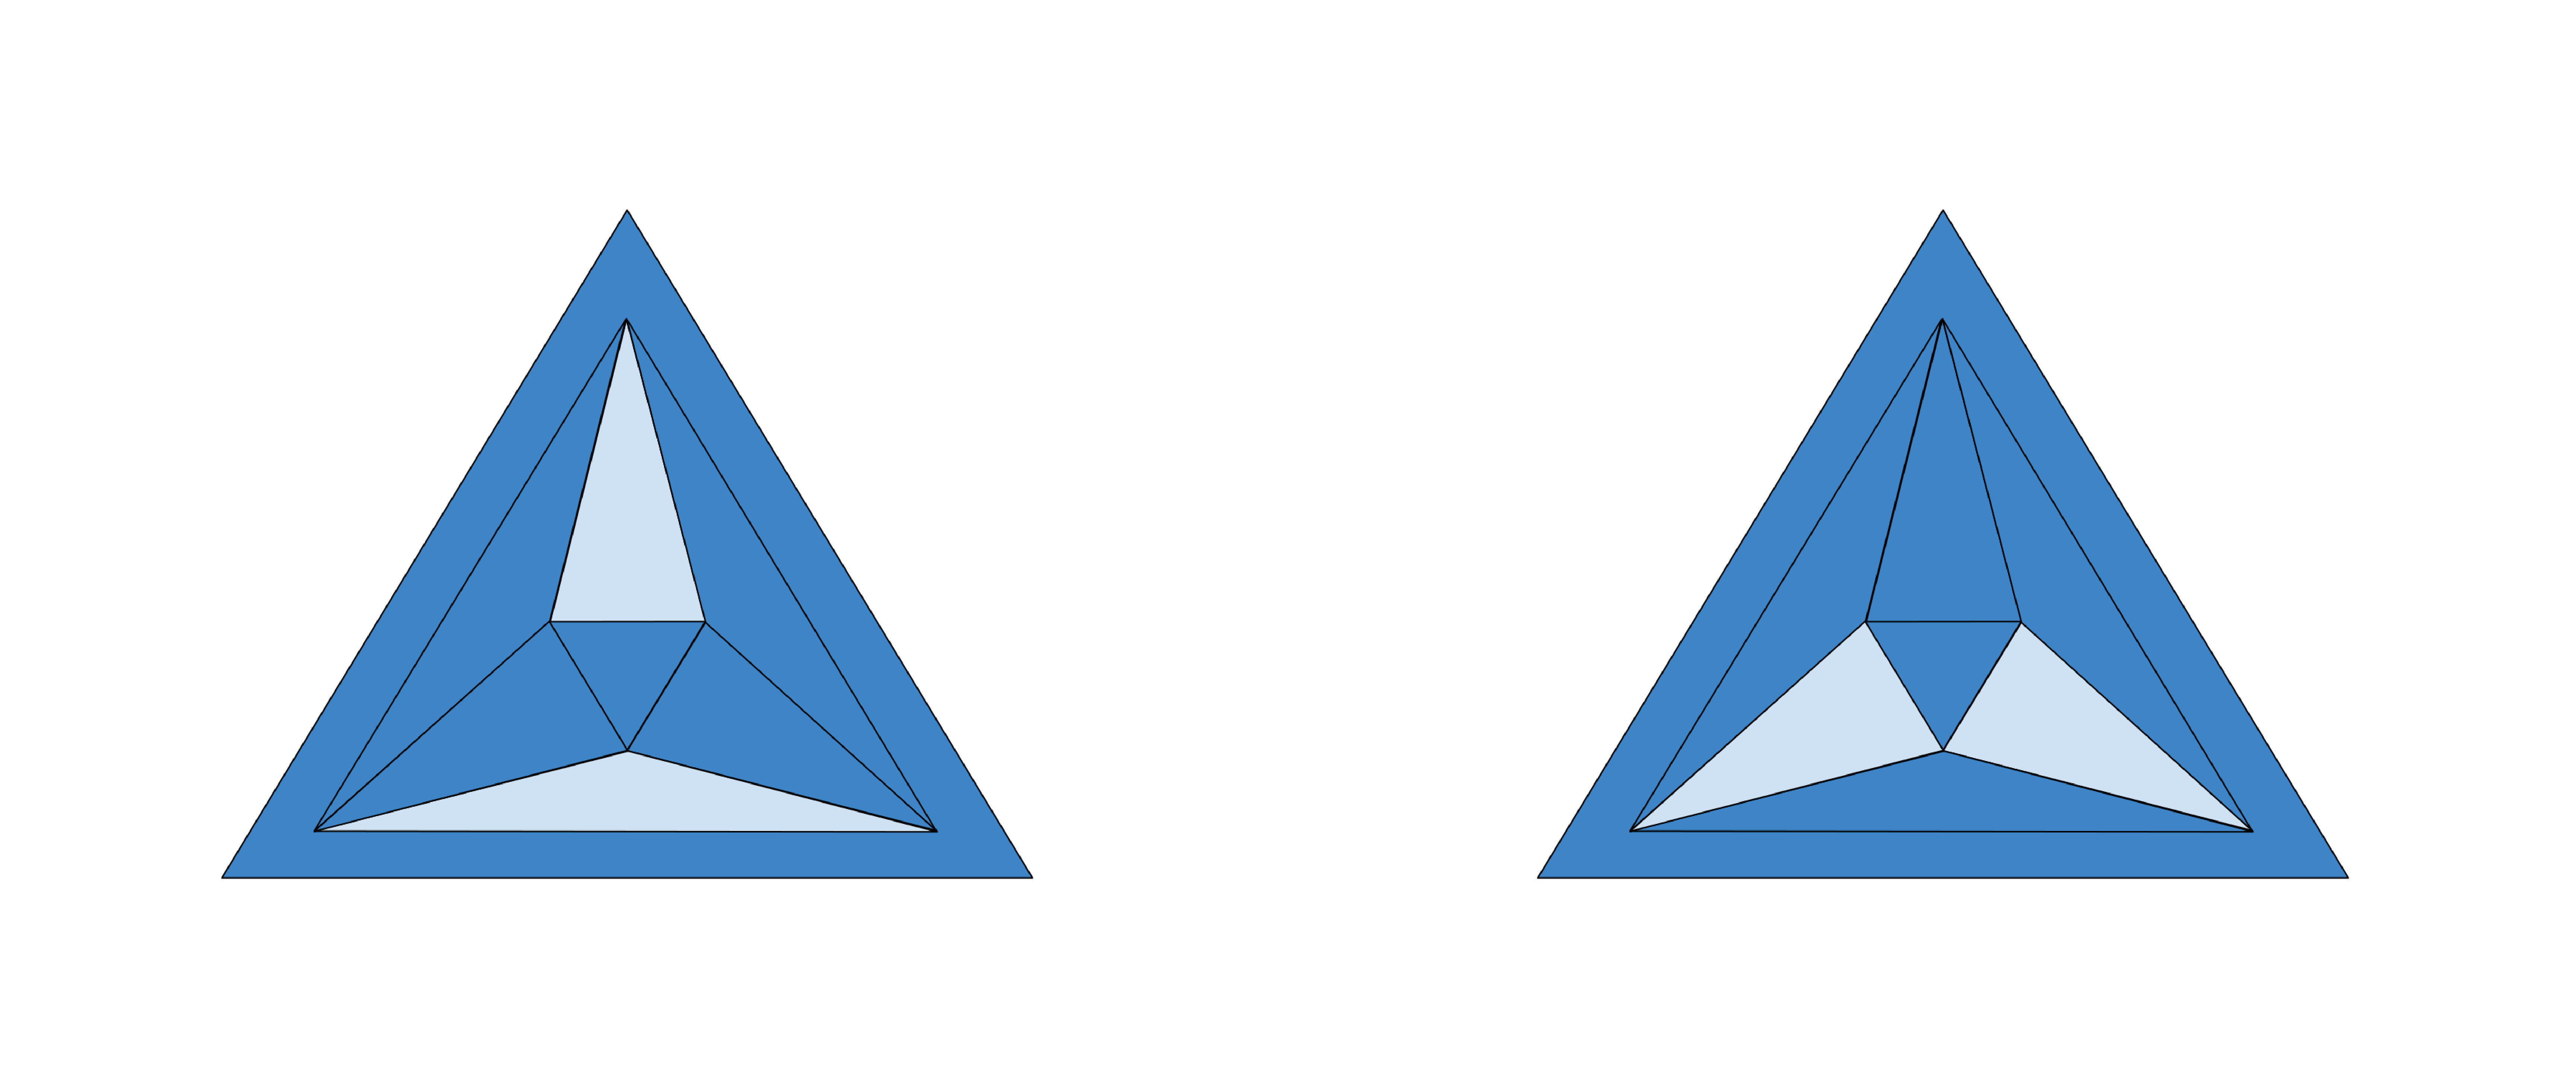
\includegraphics[scale=0.1, angle=0]{octa_state_yes.eps}
\caption{Examples of octahedron states.}
  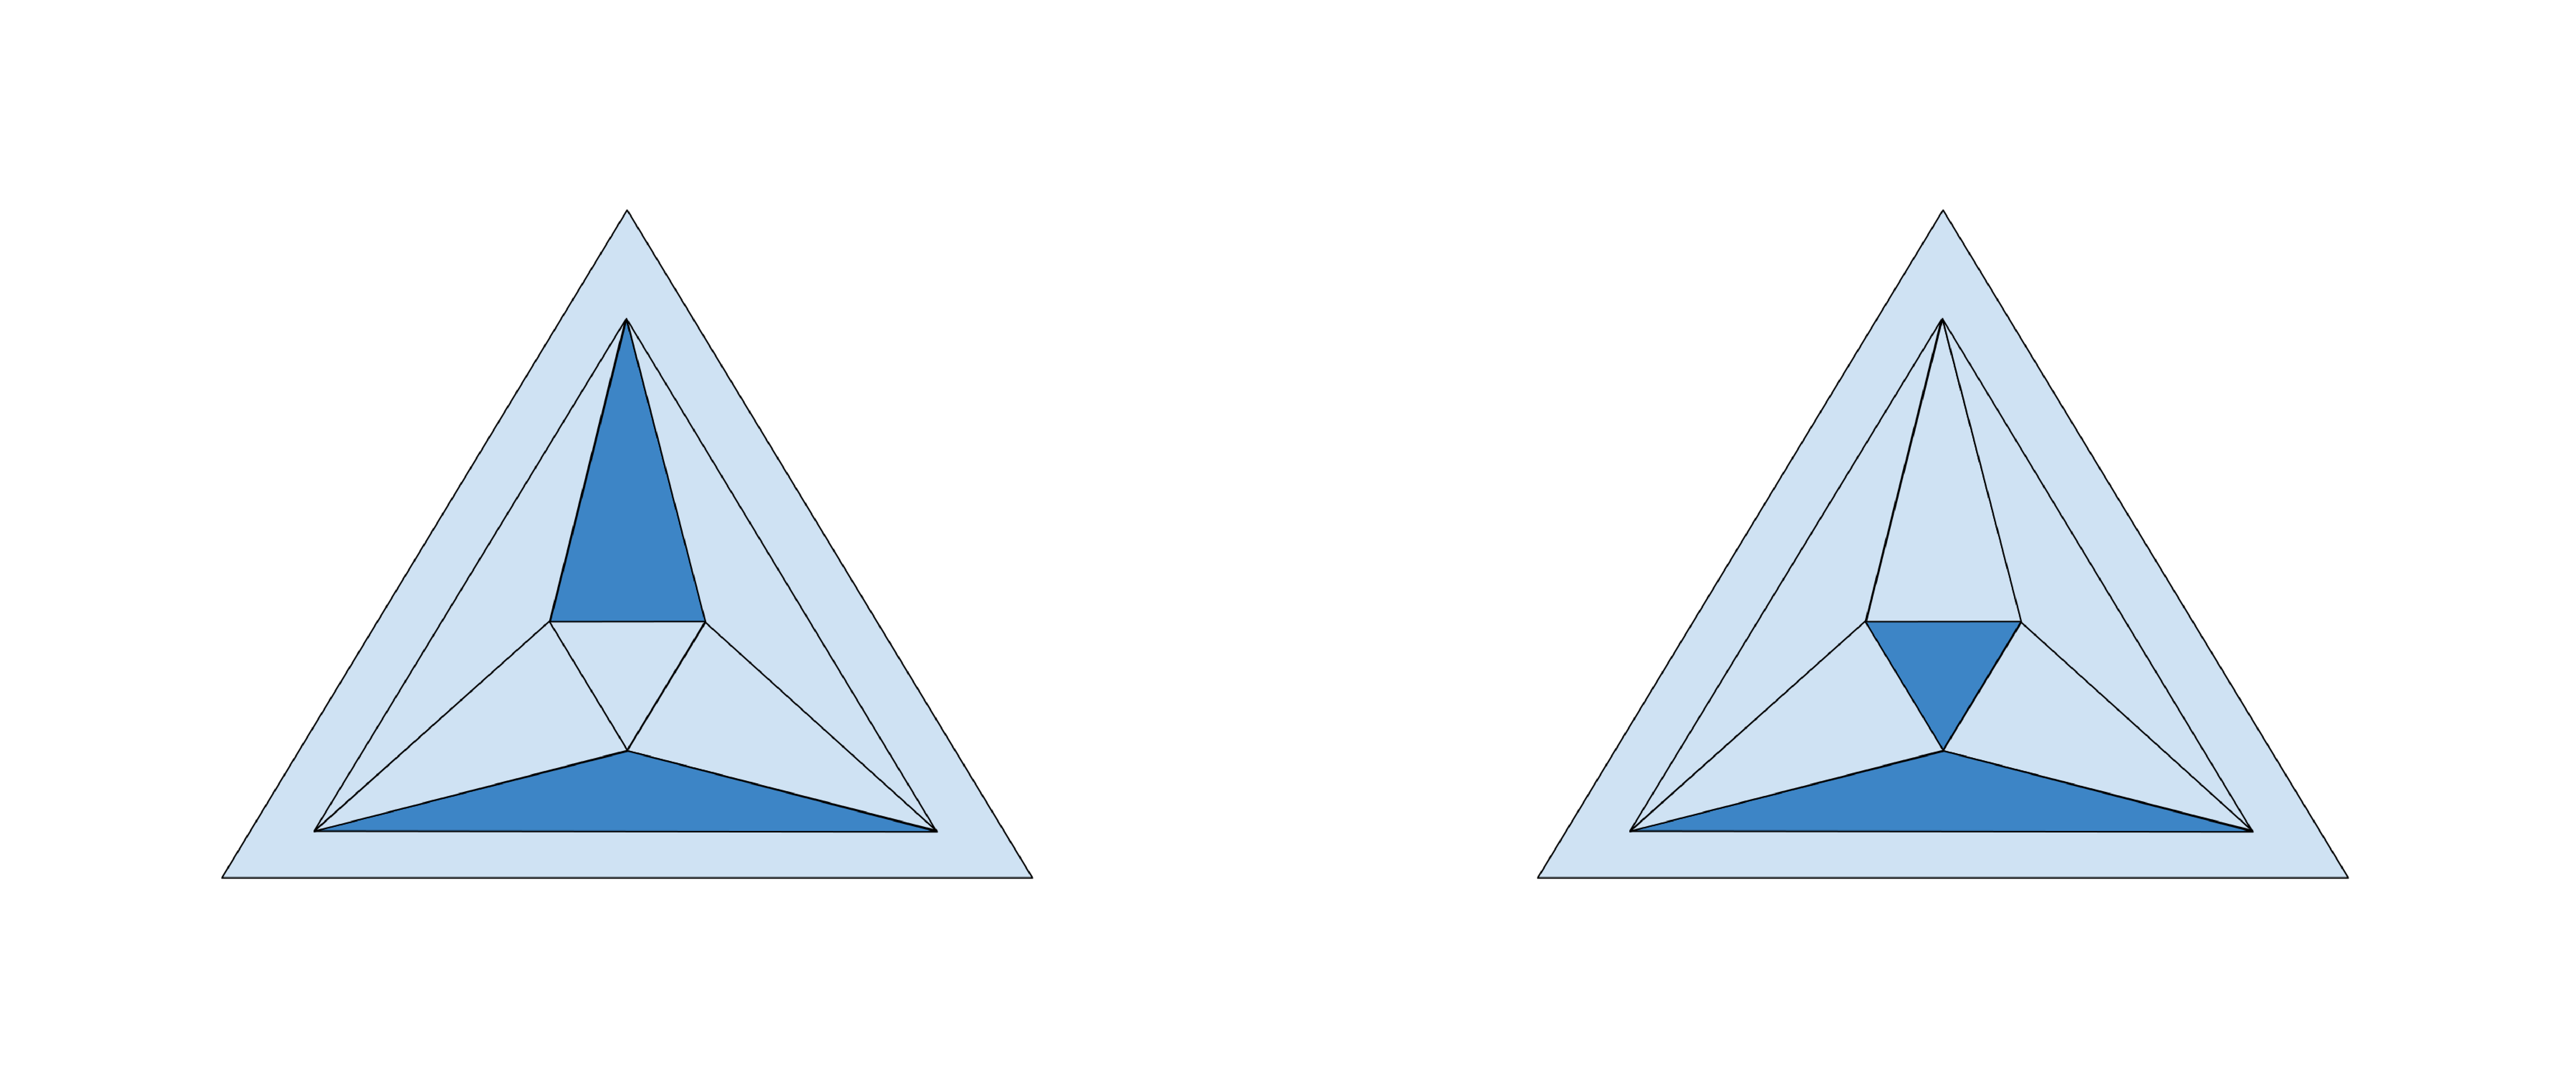
\includegraphics[scale=0.1, angle=0]{octa_state_no.eps}
\caption{Examples of octahedron non-states.}
\label{fig:OctaStates}
\end{figure}
 


%as a sequential graph labeling process. If we are interested in the BG of a polyhedron \poly, we represent \poly\spc by a graph $\PolyGraph = \left(F, E\right)$ whose nodes are the faces $F$ of \poly\spc and connections $E$ correspond to the pairs of faces sharing an edge of \poly. In this way, $\PolyGraph$ can be viewed as the polyhedral graph of \poly's dual polyhedron. 
 
%In Zlotnick's usage of the model, the labeling of $1$ or $0$ to each face would correspond to whether the face had been attached at some point up to the current step of the process. 

%--More describing fig and what is and is not an intermediate.

%The corresponding $\PolyGraph$ representation is the octahedral graph with 6 vertices and 12 edges. In this example, the state represented labels three faces with a 1 and the others with 0. The embedded geometric interpretation shows three square faces connected along their edges.

%\begin{figure}[ht]
%  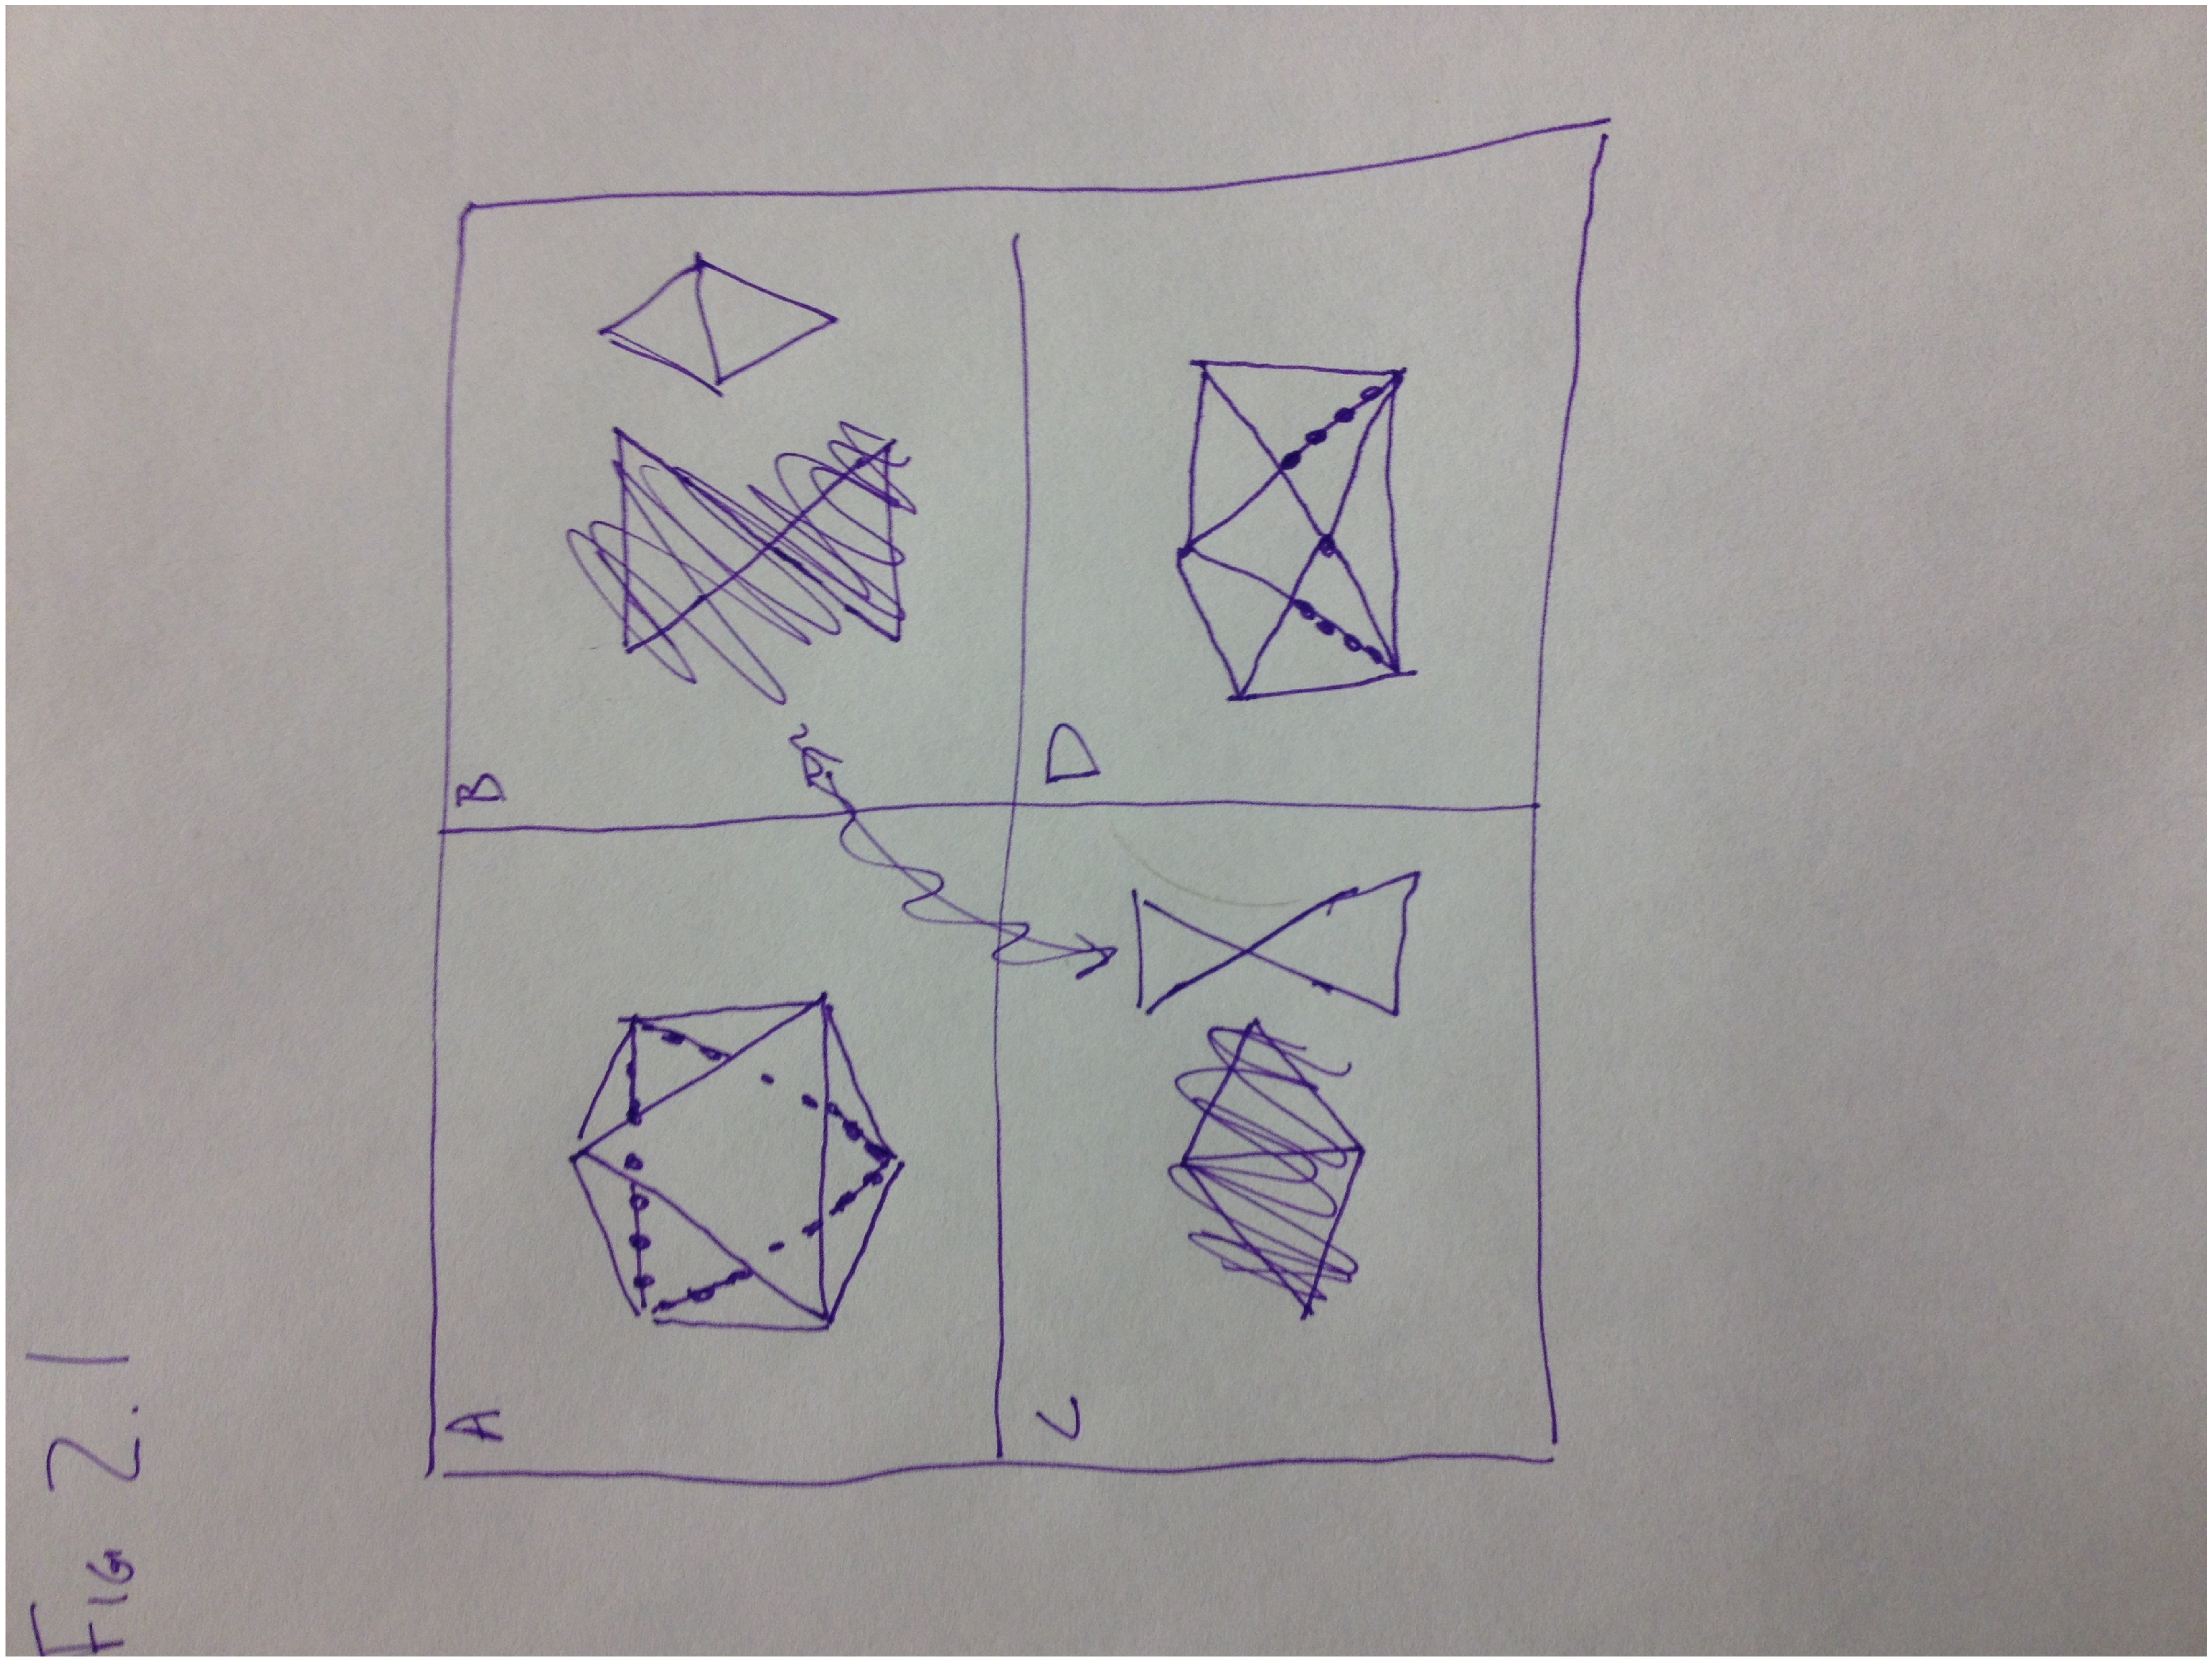
\includegraphics[scale=0.1, angle=0]{fig_2_1.eps}
%\caption{The cube and its graph representation.}
%\label{fig:OctaStates}
%\end{figure}

%\begin{mydef}
%The Building Game \textbf{rotation group} $\G$ is the permutation group acting on $F$ that corresponds to \poly's rotational symmetry group.
%\end{mydef}


\subsection{Group Actions}

It is easy to see that many states are combinatorially equivalent and are just rotations of each other. As in Endres et al., we group the states into sets that are rotations of each other~\cite{Endres2005}. However, to do so, we must first build the mathematical infrastructure using group actions. 

\begin{mydef}%[~\cite{Rotman1995}]
A \textbf{group action} of a group $G$ on a set $X$ is a function mapping $G \times X$ to $X$ with $(g, x) \mapsto g.x$ that satisfies: (i) $(gh).x = g.(h.x)$ for $g,h \in G$ and (ii) $e.x = x$ for $e$ the identity element of $G$~\cite{Rotman1995}.
\end{mydef}

We typically use a polyhedron's rotation group or one of its subgroups as $G$ and $2^F$, the set of subsets of $F$, as the set $X$ that $G$ acts on. In this case, the action $g.x$ permutes the faces of the polyhedron according to the element $g$ of the rotation group and results in a new subset of faces. Here, we introduce the concepts of orbits and stabilizer subgroups as they play an important role in our later analyses. 
\begin{mydef}%[~\cite{Rotman1995}]
Let $G$ be a group acting on a set $X$, the \textbf{orbit} of an element $x \in X$ is the subset $G.x \doteq \left\{g.x : g \in G \right\}$ of $X$~\cite{Rotman1995}.
\end{mydef}
We also use the shorthand notation $[x]$ to refer to the orbit $G.x$ since an orbit can be thought of as an equivalence class under the relation $x \sim \hat{x}$ if there is a $g \in G$ such that $x = g.\hat{x}$. 
\begin{mydef}%[~\cite{Rotman1995}]
For a  group $G$ acting on a set $X$, the \textbf{stabilizer subgroup} for an element $x\in X$ is the subgroup $G_x \doteq \left\{g \in \G :g. x = x \right\}$ of $G$ that fixes $x$~\cite{Rotman1995}.
\end{mydef}
Now, we introduce three classical results of group actions that relate orbits and stabilizer subgroups and add a corollary that we will use frequently.
\begin{mythm}[Orbit-Stabilizer~\cite{Rotman1995}]
Let $G$ be a group acting on a set $X$, then for any $x \in X, |G.x| = [G:G_x]$, the number of left-cosets of $G_x$.
\end{mythm}
\begin{mythm}[Lagrange~\cite{Rotman1995}]
If $G$ is a finite group and $S \leq G$, then $|S|$ divides $|G|$ and $[G:S] = |G|/|S|$
\end{mythm}
\begin{mylem}[Burnside~\cite{Rotman1995}]
Let $G$ be a finite group acting on a set $X$, then $$|X/G| = \frac{1}{|G|}\sum_{g \in G}|X^g|$$ where $|X/G|$ is the number of orbits and $|X^g| = \{x \in X : g.x = x\}$ 
\end{mylem}

\begin{mycor}
\label{cor:OST}
Let $G$ be a finite group acting on a set $X$, then for any $x \in X$ $$|G.x| = \frac{|G|}{|G_x|}.$$
\end{mycor}
\begin{proof}
This result follows trivially from the Orbit-Stabilizer and Lagrange's theorems. 
\end{proof}

\subsection{Building Game Intermediates}

With this framework of group actions, we now formally define the principal unit of the Building Game. 
\begin{mydef}
A Building Game \textbf{intermediate} $[x] \doteq \left\{g.x : g \in G\right\}$ is the orbit of the state $x$ under the polyhedra's rotation group. 
\end{mydef}
Since the orbits of a group action form a partition on the set it acts on, each state belongs to a single intermediate and two states $x$ and $y$ are part of the same intermediate if there is a $g\in\G$ such that $y = g.x$. In the case of the tetrahedron, as pictured in figure~\ref{fig:TetraStates}, there are only four intermediates since any state with the same number of faces can be rotated to reach the others. 

%\begin{mylem}
%\label{lem:GyhGxh}
%Let $x, y \in \left[x\right]$ such that $y = h.x$ for some $h \in G$. Then, $G_y = hG_xh^{-1}$. 
%\end{mylem}
%\begin{proof}
%Since $G$ is normal to itself, we have $G = h^{-1}Gh = hGh^{-1}$.
%\begin{align}
%  hG_xh^{-1} &= \left\{hgh^{-1} : g \in G_x \right\} \\
%  &= \left\{hgh^{-1} : g.x = x, g \in G\right\} \\
%  \intertext{Use the transformation $\hat{g} = hgh^{-1}$.}
%  &= \left\{\hat{g} : h^{-1}\hat{g}h.x = x, \hat{g} \in hGh^{-1} \right\} \\ 
%  &= \left\{\hat{g} : \hat{g}.(h.x) = h.x, \hat{g} \in G \right\} \\ 
%  &= \left\{\hat{g} : \hat{g}.y = y, \hat{g} \in G \right\} \\ 
%  &= G_y
%\end{align}
%\end{proof}

Since we have defined the intermediates to be the orbits of states under the polyhedral group, we are naturally also interested in stabilizer subgroups of Building Games states.
\begin{mydef}
The \textbf{symmetry number} $r_{x^j}$ (or simply $r_j$) of a state $x^j$ is the order of its stabilizer subgroup $\left|\G_{x^j}\right|$.
\end{mydef}
In figure~\ref{fig:OctaStabs} we see three states and their orbit stabilizer subgroups. The first state, with only a single face, has a symmetry number of $3$ since any rotation by a multiple of $\frac{2\pi}{3}$ fixes the face. The second has a symmetry number of $2$ since only the identity and a rotation by $\pi$ will fix the faces. The final state, with three faces, cannot be fixed by any rotation other than the identity and thus has symmetry number $1$.  
\begin{figure}[ht]
        \centering
  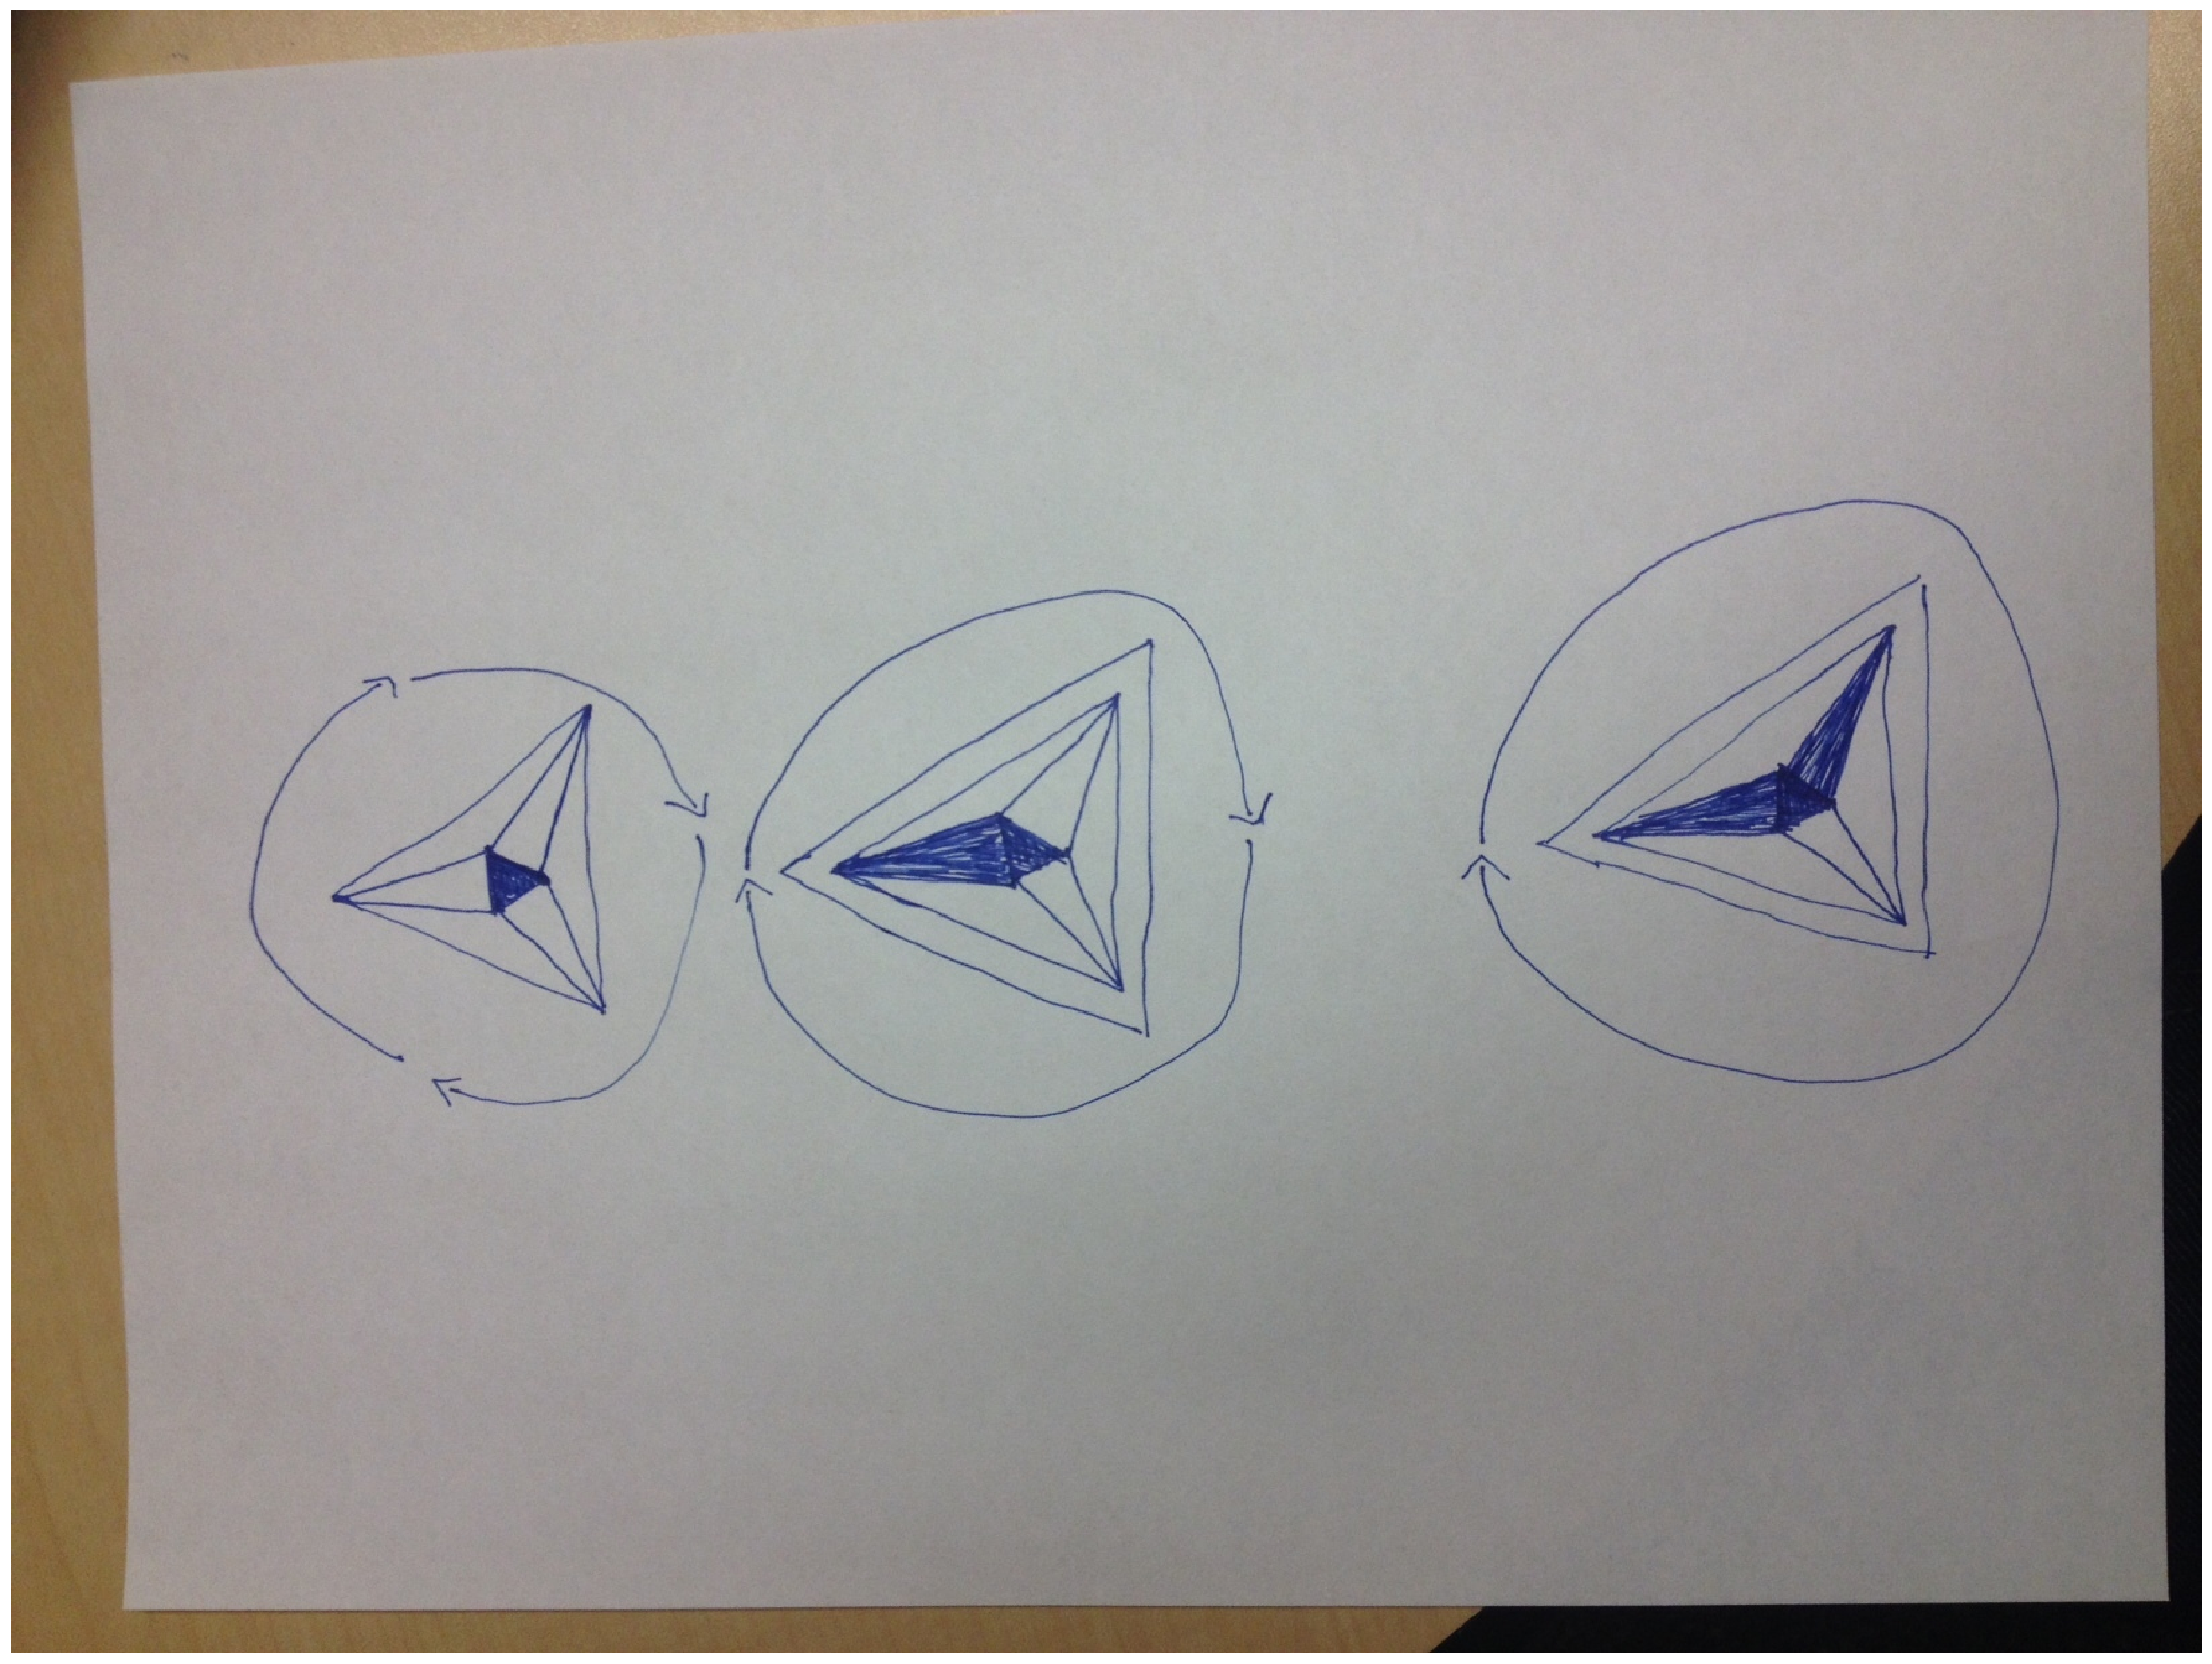
\includegraphics[scale=0.08, angle=0]{octa_stabilizers.eps}
\caption{The stabilizer subgroups for various octahedron states.}
\label{fig:OctaStabs}
\end{figure}

\begin{mythm}
If the states $x$ and $\hat{x}$ are members of the same intermediate $\left[x\right]$, they have the same symmetry number. Thus, we extend the notion of a symmetry number to be a property of an intermediate.
\end{mythm}
\begin{proof}
By Corollary~\ref{cor:OST} and since $G.x \doteq [x] = [\hat{x}] \doteq G.\hat{x}$, the result follows.
\begin{align}
  r_x &= |G_x| \\
  &= \frac{|G|}{|G.x|} \\
  &= \frac{|G|}{|G.\hat{x}|} \\
  &= |G_{\hat{x}}| \\
  &= r_{\hat{x}}
\end{align}
\end{proof}


%\begin{figure}[ht]
%\caption{The eight states in a particular BG intermediate.}
%\label{fig:CubeState}
%\end{figure}

%For ease of exposition, we use the notational shorthand $\left(x\right)_m$ for $x\left(f_m\right)$ and $x = g.x'$ when $x(f_m) = x'(g.f_m)$ for every $f_m \in F(\mathscr{P})$. Additionally, we denote the intermediate satisfying $\left(x\right)_m = \colorA$ for all $f_m \in \faceset$ as $x^\colorAsm$ and similarly $x^\colorBsm$ is the intermediate with $\left(x\right)_m = \colorB$ for all $f_m \in \faceset$. The function counting the number of \colorB\spc faces an intermediate has is denoted $h\left(x\right) \doteq |\left\{f_m \in \faceset : \left(x\right)_m = \colorB\right\}|$.

Since the Building Game is at its core an attachment model, we are interested in which intermediates can be formed from others by attaching a face to a particular intermediate.
\begin{mydef}
Two distinct intermediates $\left[x\right]$ and $\left[y\right]$ are \textbf{connected} if there exist states $x \in \left[x\right]$ and $y \in \left[y\right]$ such that one of the following holds:
\begin{itemize}
 \item there is a face, $f$, in the state $y$ such that $y = x \cup \left\{f\right\}$
 \item there is a face, $f$, in the state $x$ such that $x = y \cup \left\{f\right\}$
\end{itemize}
\end{mydef}

\begin{mylem}
If intermediates $\left[x\right]$ and $\left[y\right]$ are connected, then for every state $x \in \left[x\right]$ there is a state $y \in \left[y\right]$ such that $\exists f \in y: y = x \cup \left\{f\right\}$ or $\exists f \in x: x = y \cup \left\{f\right\}$.
\end{mylem}
\begin{proof}
  Without loss of generality, assume $|x| < |y|$. Since $[x]$ and $[y]$ are connected, let $\hat{x} \in [x]$, $\hat{y} \in [y]$, and $\hat{f} \in \hat{y}$, be such that $\hat{y} = \hat{x}\cup\{\hat{f}\}$. Then, for any $x \in [x]$, pick $g \in G$ such that $x = g.\hat{x}$. By choosing $y = g.\hat{y}$ and $\{f\} = g.\{\hat{f}\}$, we have
\begin{align}
  y &= g.\hat{y} \\
  &= g.(\hat{x}\cup\{\hat{f}\}) \\
  &= g.\hat{x}\cup g.\{\hat{f}\} \\
  &= x \cup \{f\} \\
\end{align}    
and our result is shown.
\end{proof}


\begin{mydef}
A Building Game \textbf{pathway} is a sequence of intermediates $[x^{p_1}], [x^{p_2}], \dots, [x^{p_N}]$ such that  $[x^{p_i}]$ is connected to $[x^{p_{i+1}}]$, $|x^{p_i}| = i$, and $x^{p_N} = F$.
\end{mydef}

 Figure~\ref{fig:OctaPath} shows a Building Game pathway for the octahedron using Schlegel diagrams. The pathway has $8$ intermediates since there must be exactly one intermediate $x^{p_i}$ satisfying $h\left(x^{p_i}\right) = i$ for each $i = 1,2,\dots,8$.

\begin{figure}[ht]
\centering
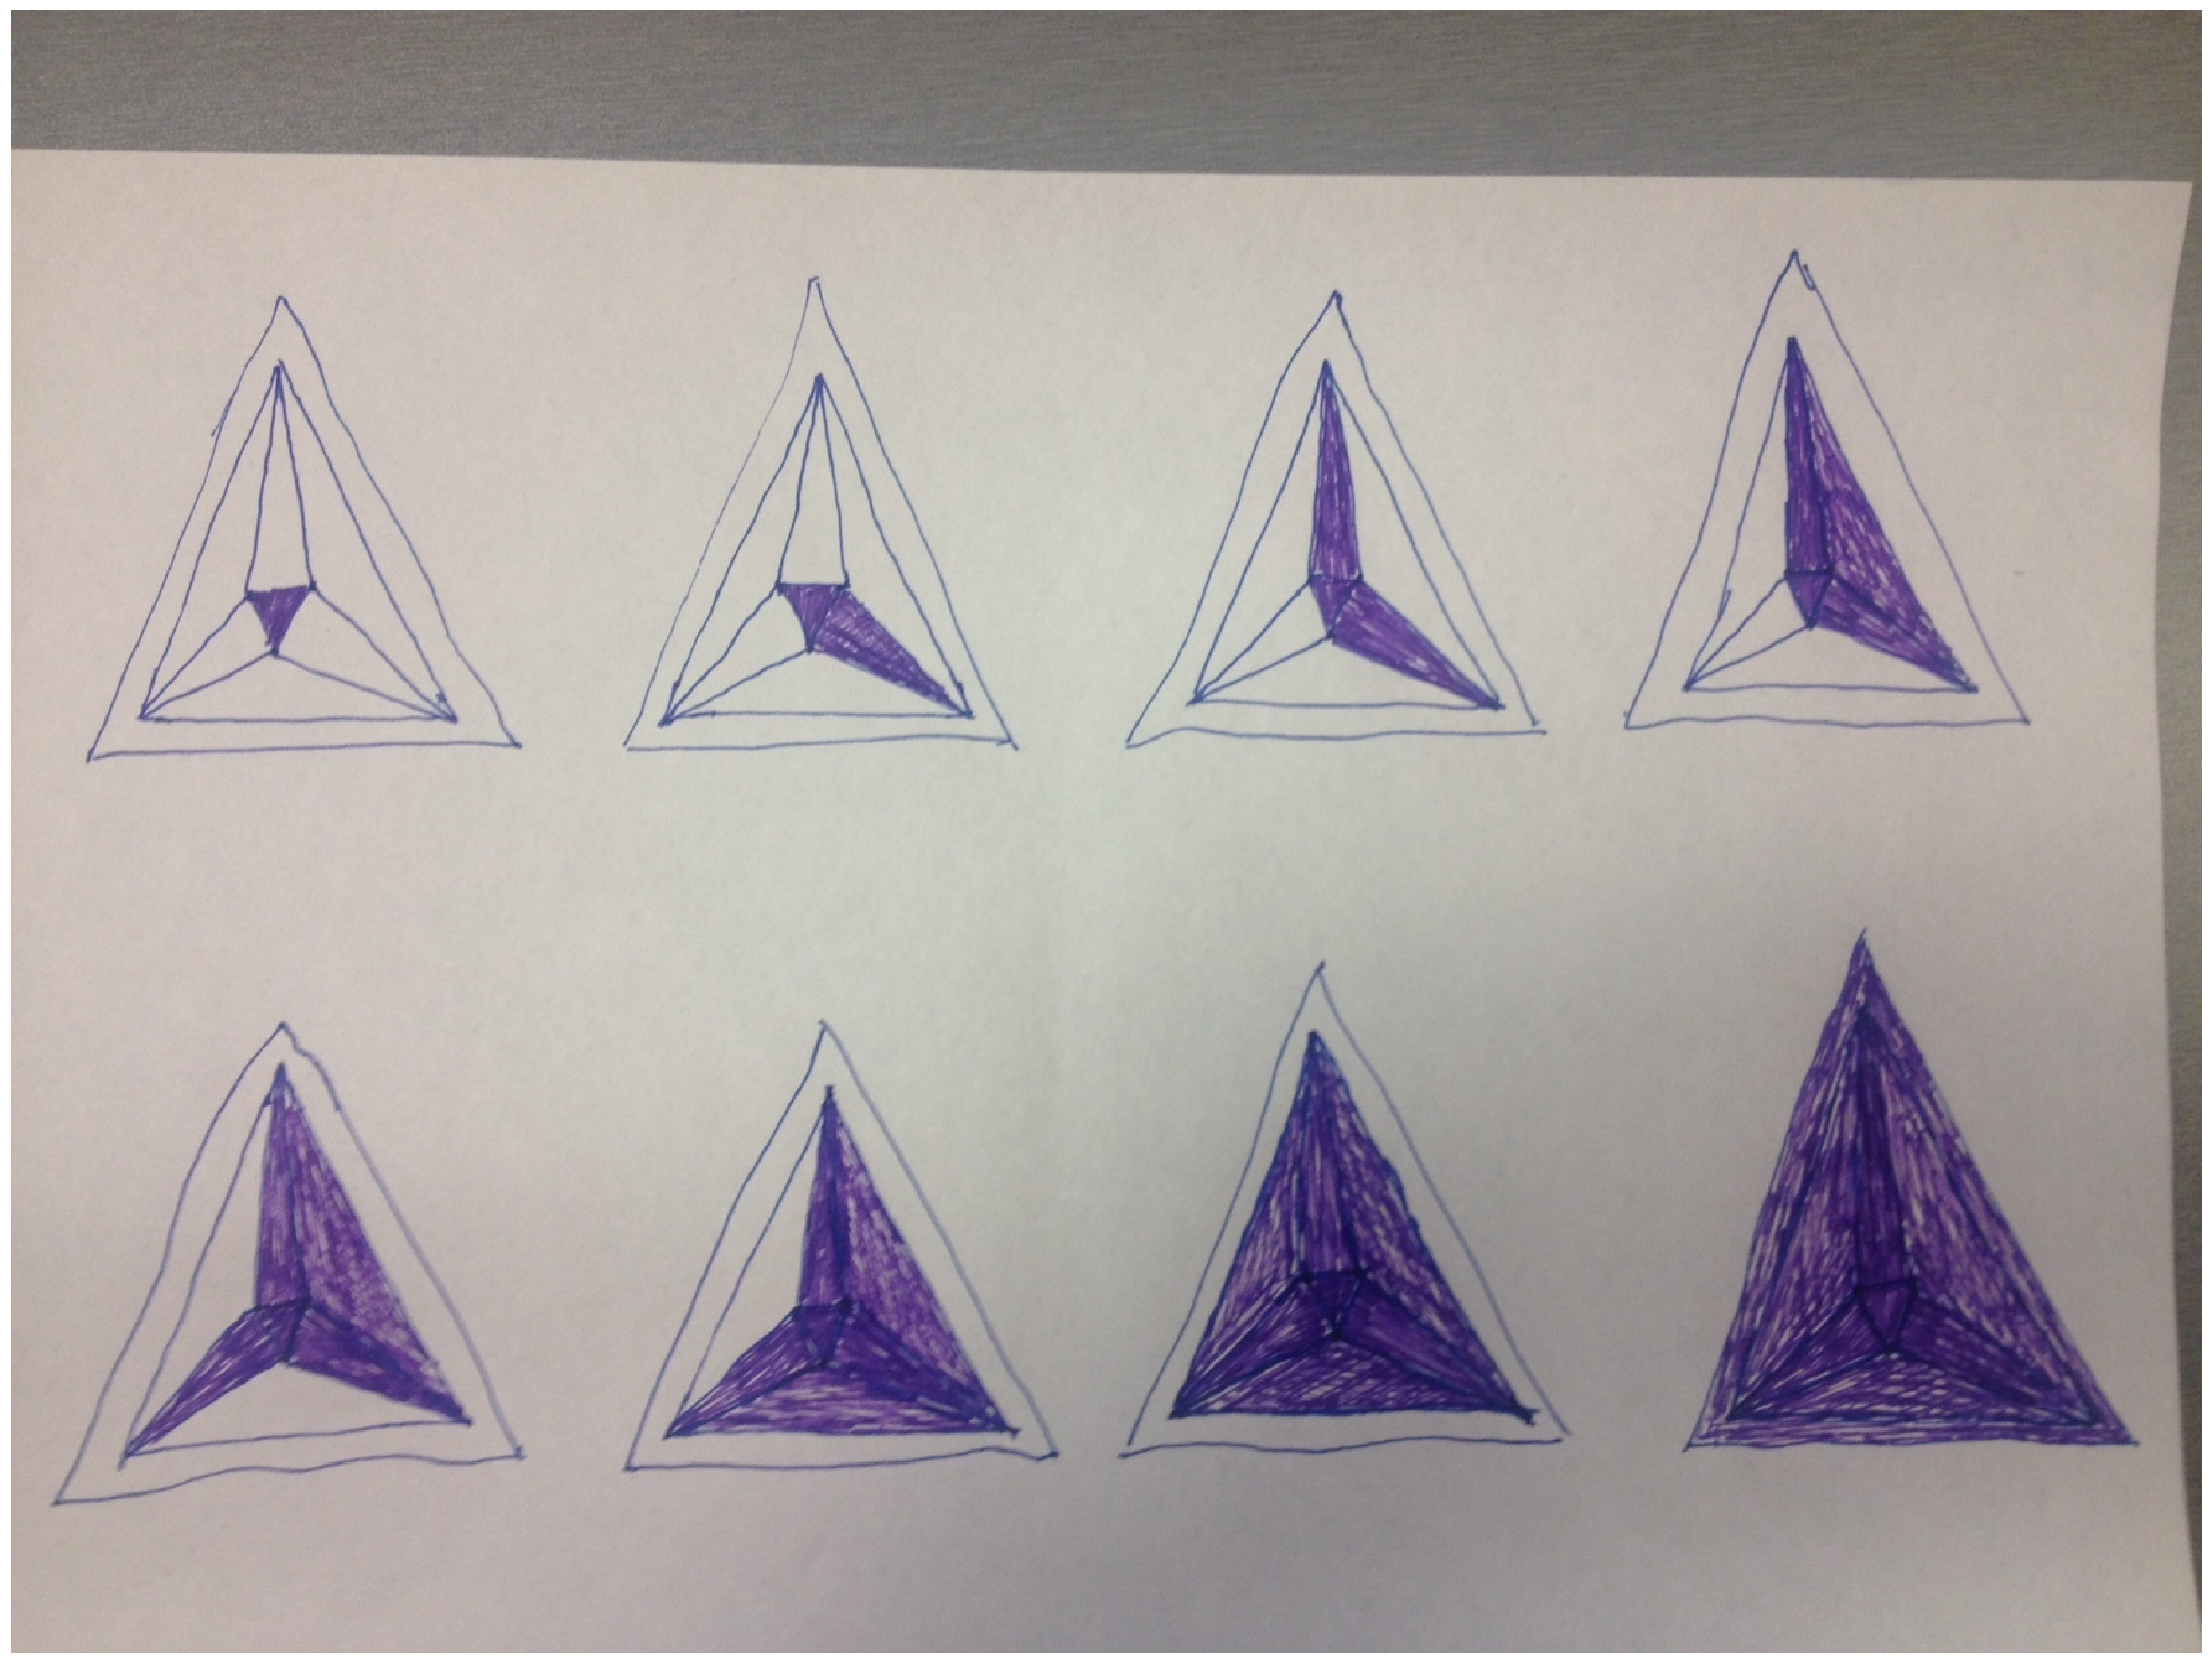
\includegraphics[scale=0.065, angle=0]{octa_path.eps}
\caption{One Building Game pathway for the Octahedron.}
\label{fig:OctaPath}
\end{figure}

\begin{mydef}
The Building Game \textbf{combinatorial configuration space} for a polyhedron is a graph in which the nodes are the polyhedron's intermediates and a graph edge exists between two intermediates if and only if they are connected. 
\end{mydef}

When the intermediates are partitioned by the number of faces they possess, it is natural to arrange the combinatorial configuration space into columns or tiers according to this partition. Figure~\ref{fig:CubeCCS} shows the Building Game state space for the cube. As seen, each column has intermediates with the same number of faces and connections thus exist with intermediates that are either in the tier directly above or below them. We can also see that there are three distinct pathways contained in the state space. 

\begin{figure}[ht]
\centering
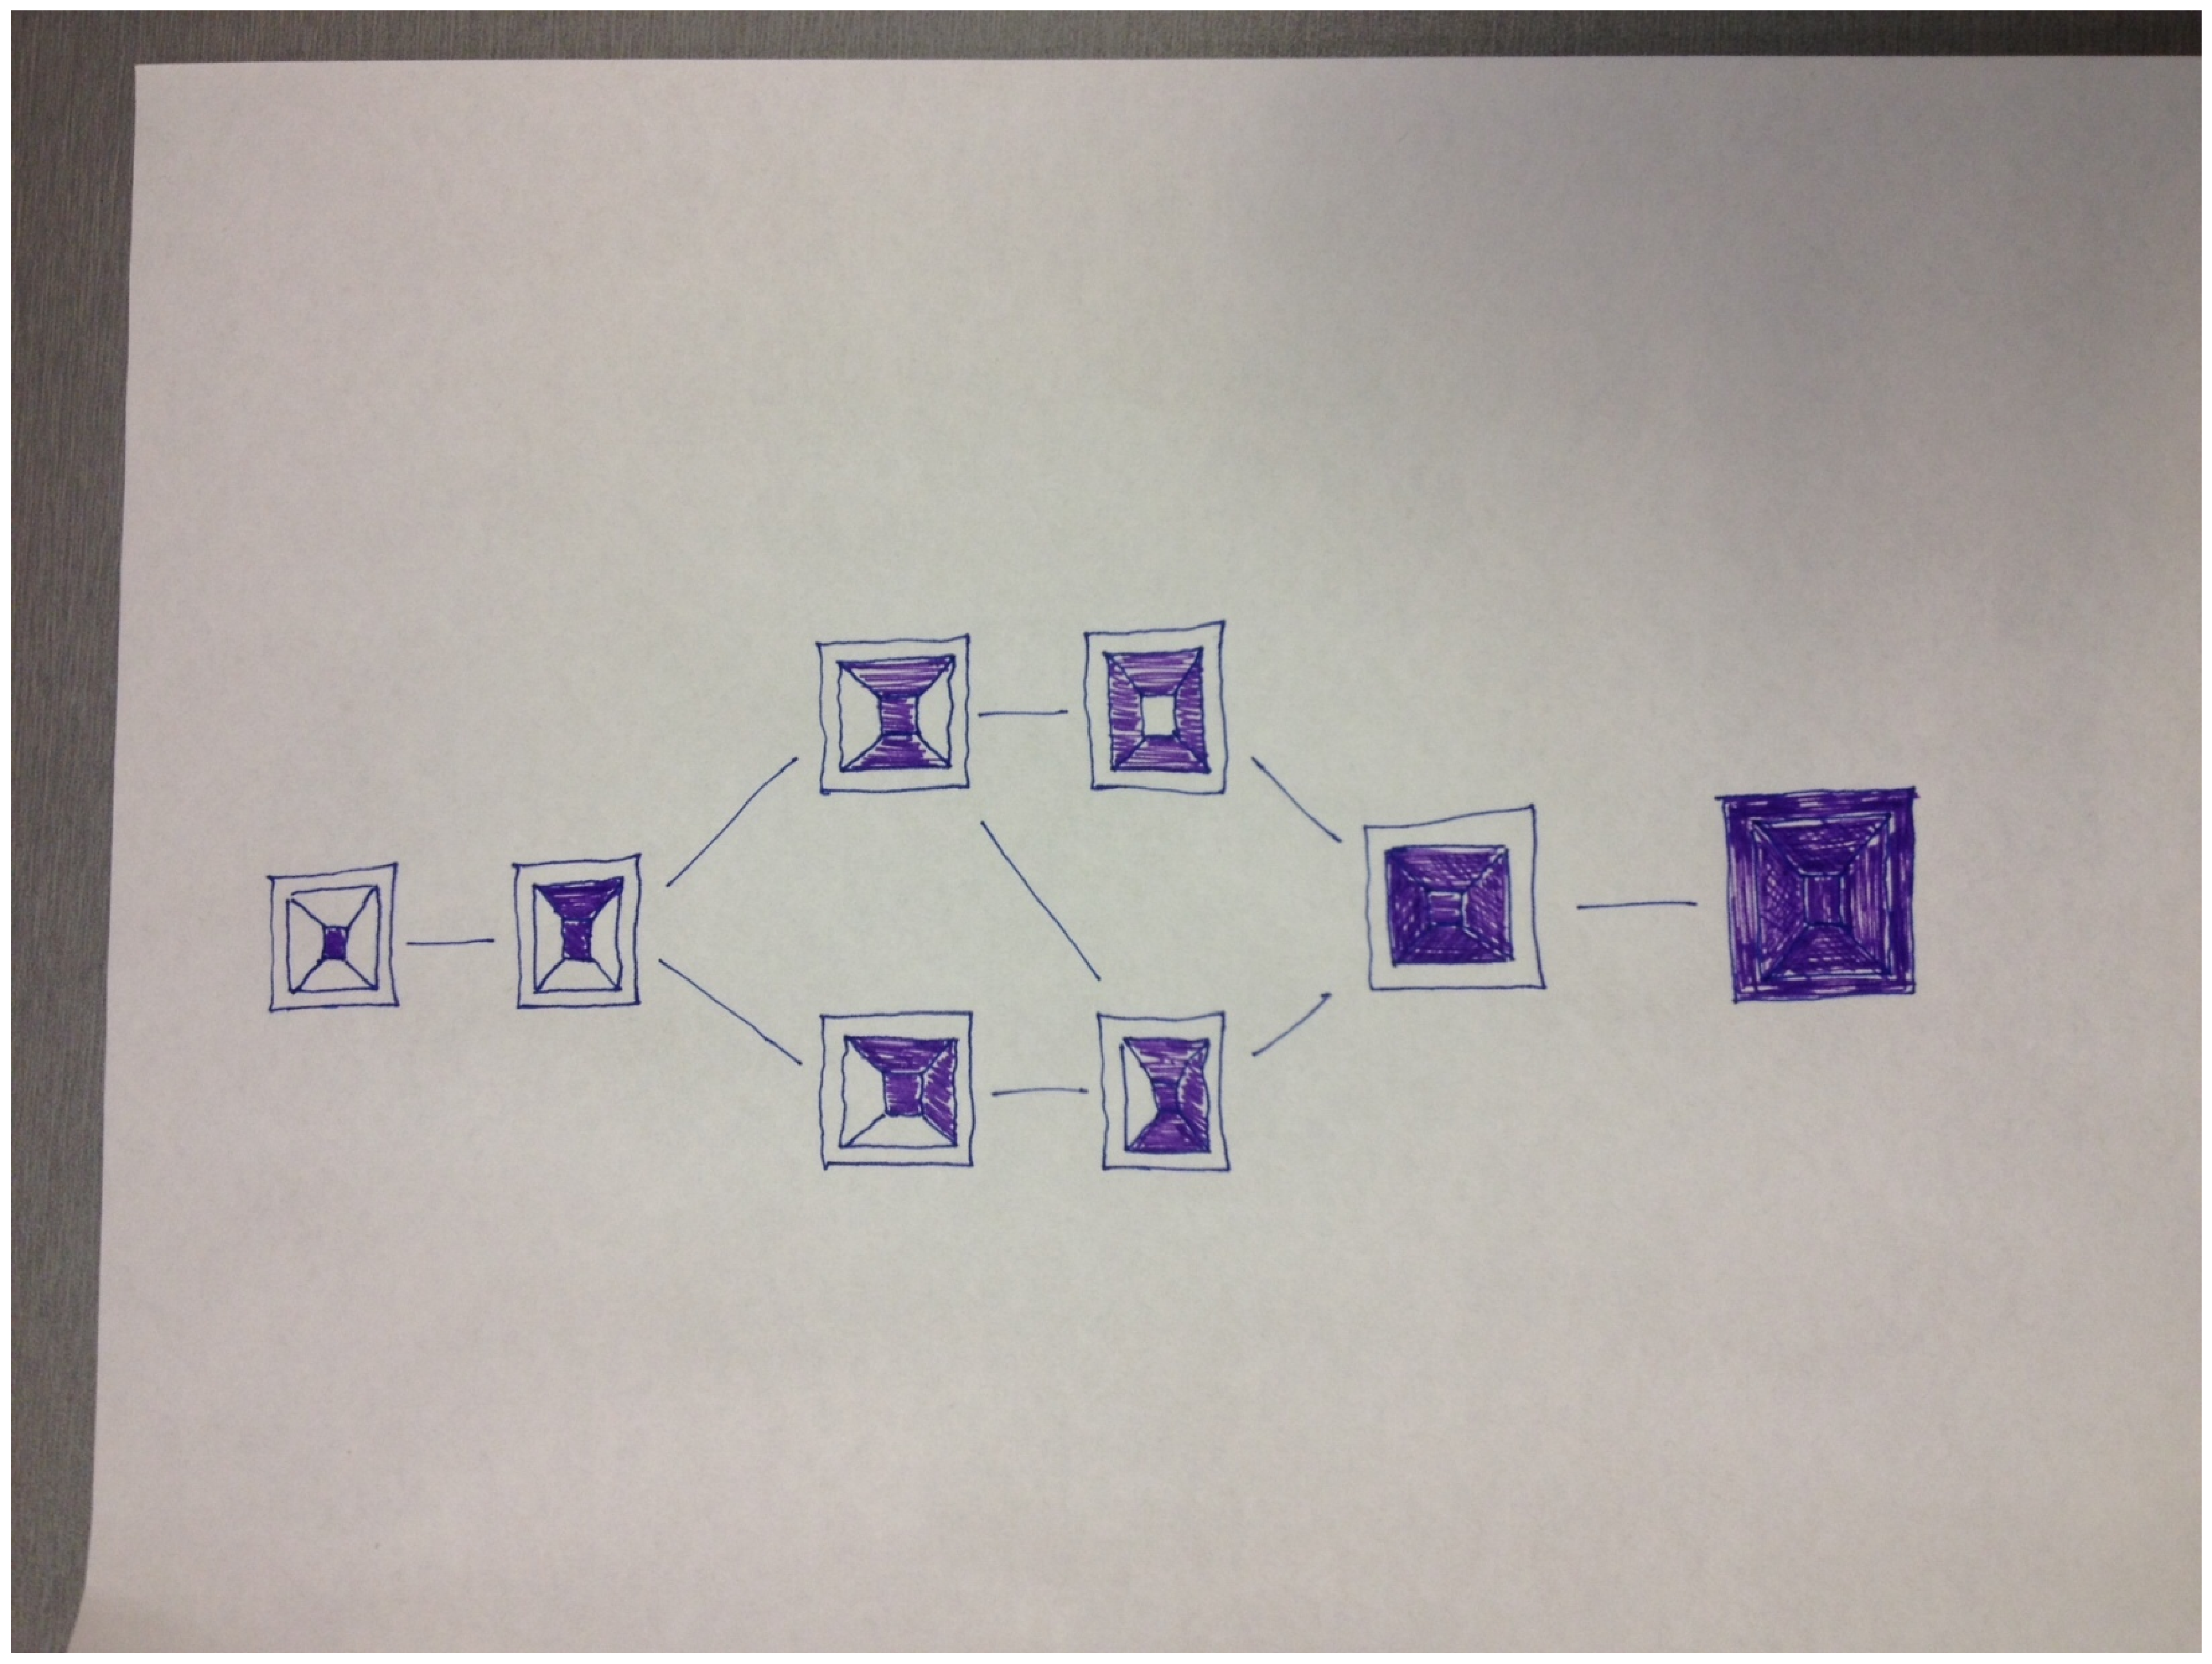
\includegraphics[scale=0.2, angle=0]{cube_ccs.eps}
\caption{The Building Game combinatorial configuration space of the cube.}
\label{fig:CubeCCS}    
\end{figure}

Interestingly, it is not the case that the addition or removal of each face of an intermediate results in a distinct intermediate. 
\begin{mydef}
For two connected intermediates $[x^j]$ and $[x^k]$, the set of different faces $$F_{jk} \doteq \left\{f \notin x^j : x^j\cup\{f\} \in [x^k]\right\}\cup\left\{f \in x^j : x^j\setminus\{f\} \in [x^k]\right\}$$ that can be added or removed from $x^j$ to get an element of $[x^k]$ is called the \textbf{degeneracy set} and the number of such faces $S_{jk} \doteq \left|F_{jk}\right|$ is called the \textbf{degeneracy number}.
\end{mydef}

The act of attaching an additional face is referred to as a forward step in the Building Game and the removal of a face is a backward step. As such, degeneracies are sometimes referred to as forward or backward degeneracies. It is important to note that in general the degeneracy number is not symmetric, i.e. \Sjk$\neq$\Skj\spc for some connections $[x^j] \leftrightarrow [x^k]$ in the state space. Figure~\ref{fig:CubeDegen} depicts the forward and backward degeneracy numbers for a particular connection. As illustrated, there are four faces that can be added to the first intermediate to form the second. However, removing any of the two faces of the second intermediate will result in the first. Thus the forward degeneracy number is four and the backward degeneracy number is two.  


\begin{figure}[ht]
\centering
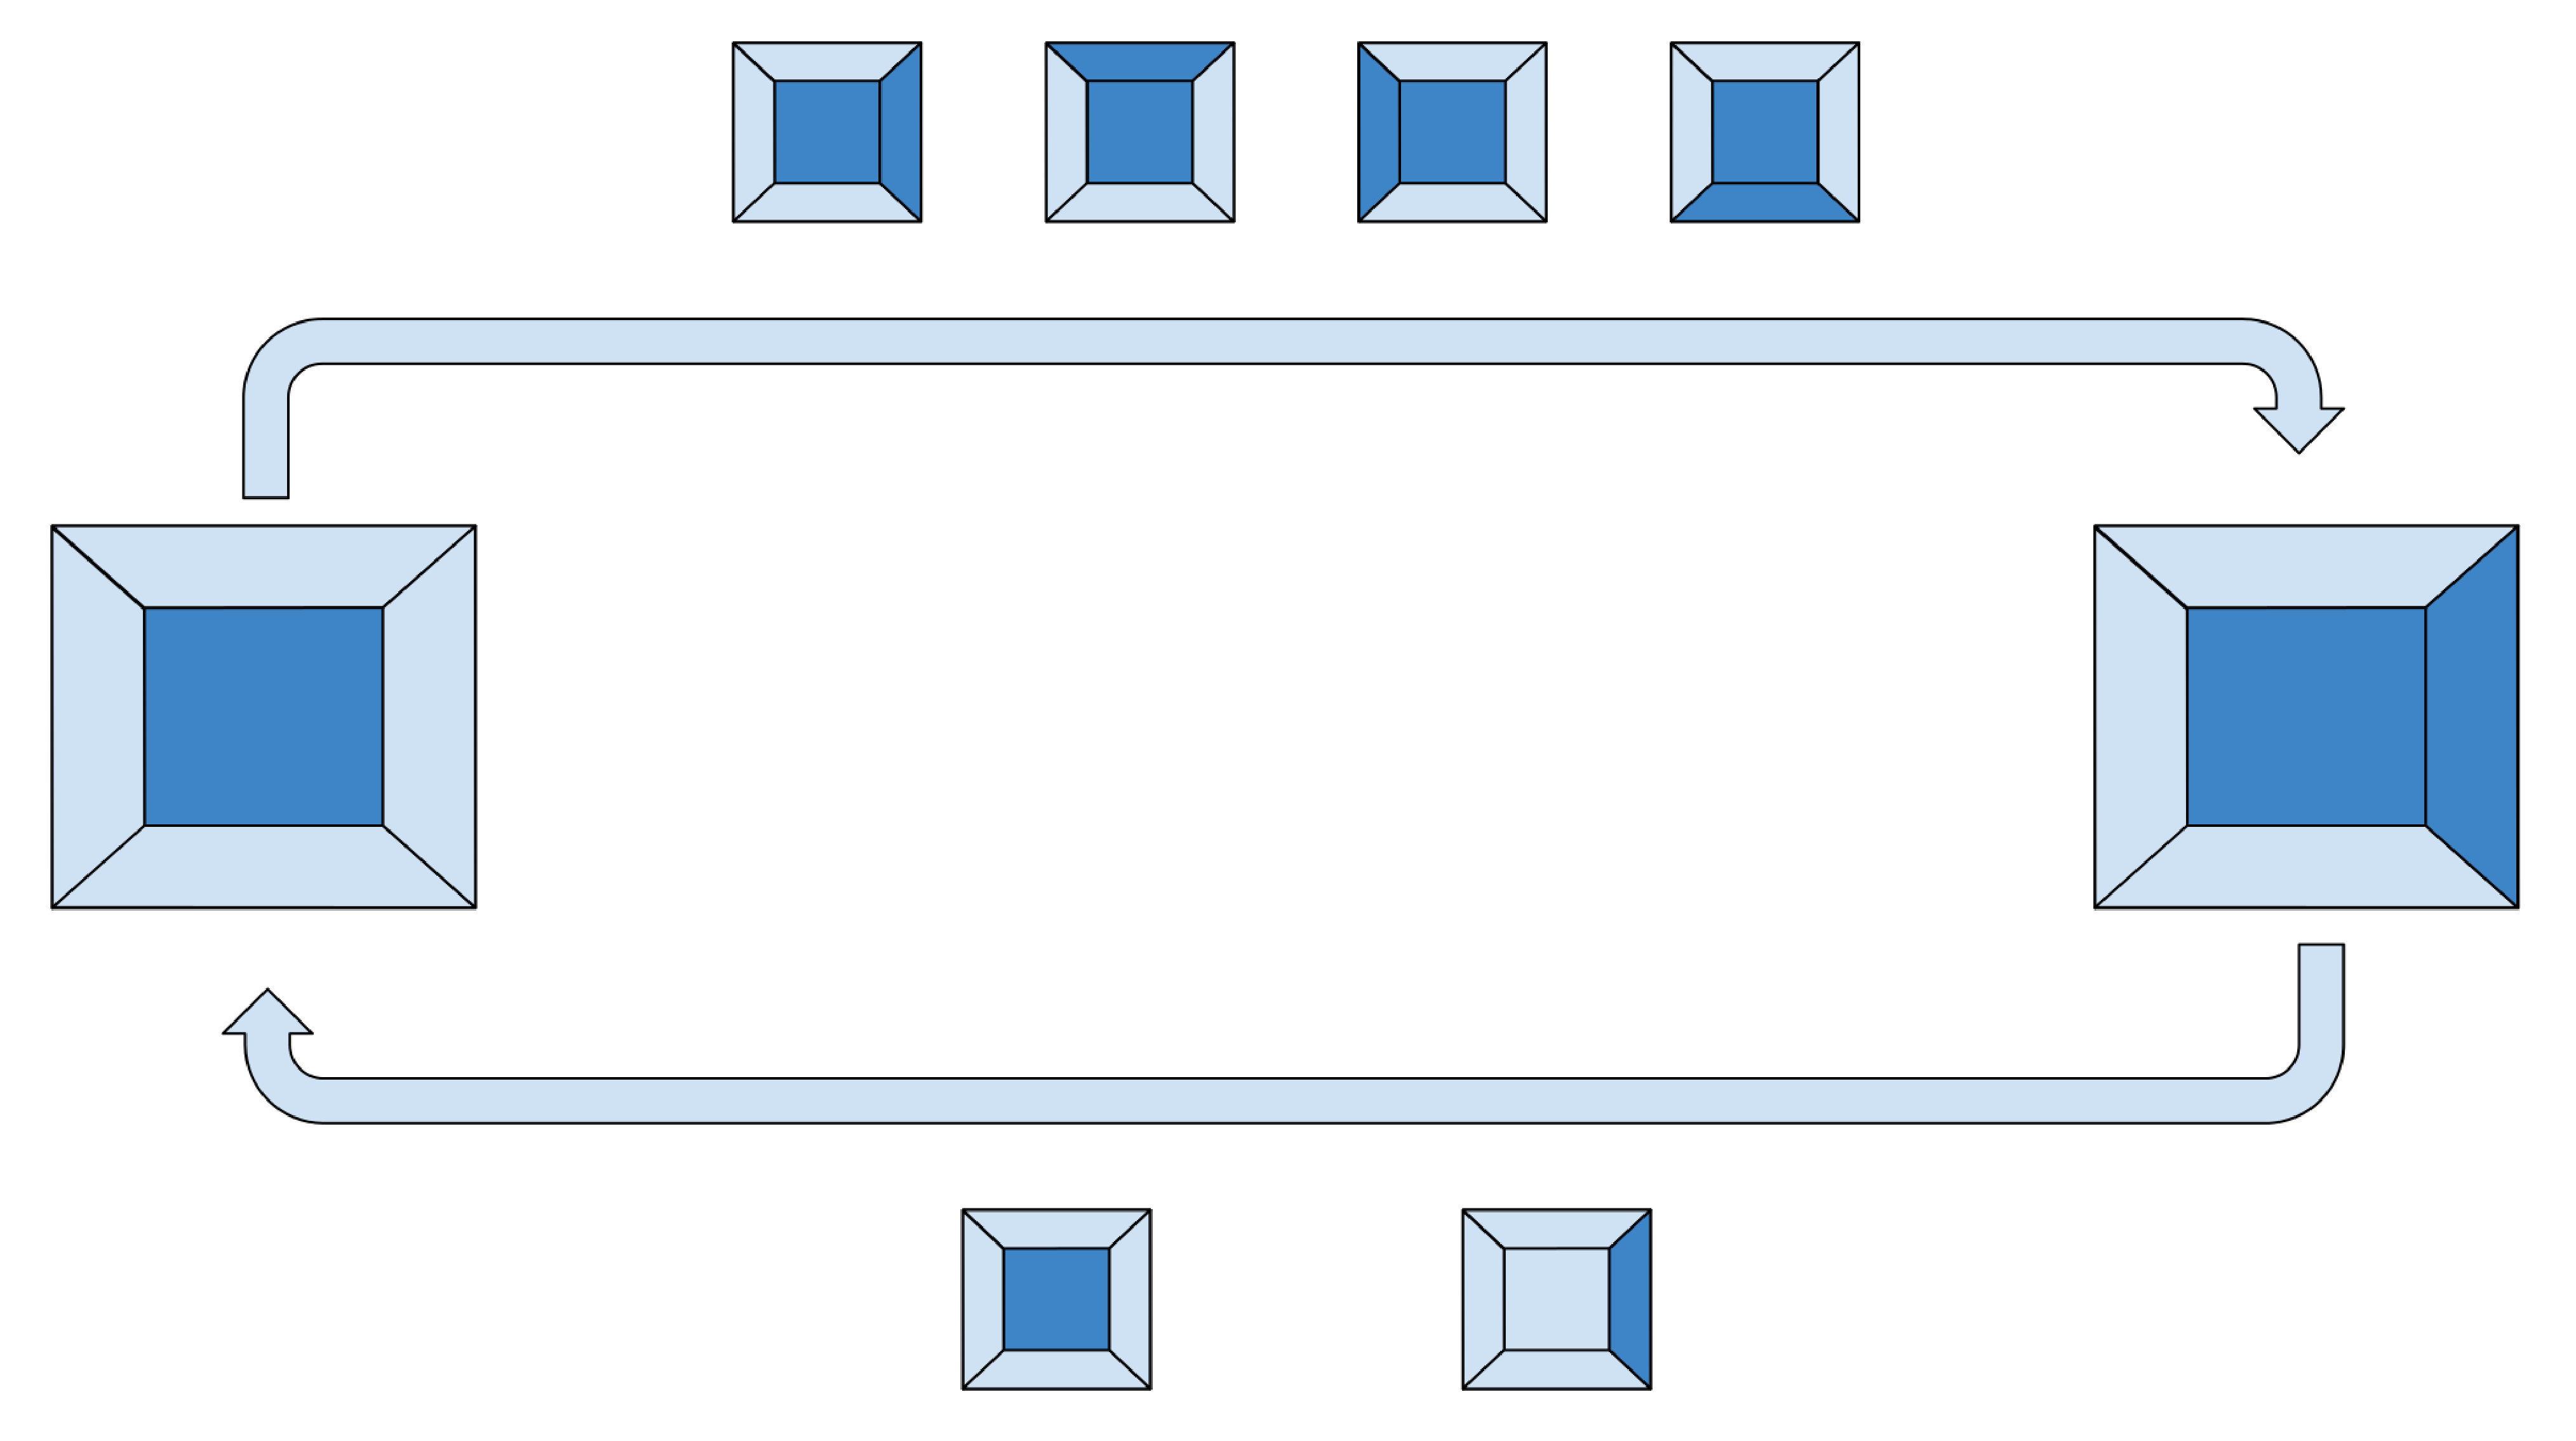
\includegraphics[scale=0.17, angle=0]{cube_degens.eps}
\caption{Degeneracies between two connected cube intermediates.}
\label{fig:CubeDegen}    
\end{figure}


Finally, we extend the notion of a pathway to to be a sequence of intermediates of arbitrary lengths, such that the sequence begins at an intermediate with a single face and ends with the completed polyhedron and each pair of successive intermediates are connected.
\begin{mydef}
A Building Game \textbf{reversible pathway} is a sequence of intermediates $[x^{p_1}], [x^{p_2}], \dots, [x^{p_N}]$ such that  $[x^{p_i}]$ is connected to $[x^{p_{i+1}}]$, $|x^{p_0}| = 1$, and $|x^{p_N}| = |F|$.
\end{mydef}


%\begin{mythm}
%  For two connected intermediates $[x^j]$ and $[x^k]$, the degeracy numbers $S_{jk}$ and $S_{kj}$ are that same as the cardinality of $G_{x^j}.\{f\}$ and $G_{x^k}.\{f\}$ for $x^j \in [x^j], x^k \in [x^k], f \in F$ satisfying $x^k = x^j \cup \{f\}$.  
%\end{mythm}
%\begin{proof}
%
%First we argue the case of $S_{jk}$ by showing that $G_x^j.\{f\} = \{\hat{f} \in F : x \cup \{\hat{f}\} \in [y]\}$.
%
%Assume $\{\hat{f}\} \in G_{x^j}.\{f\}$. Thus, there is a $g \in G$ such that $g.x = x$ and $g.\{f\} = \{\hat{f}\}$. It follows that
%\begin{align}
%x \cup \{\hat{f}\} &= (g.x)\cup (g.\{f\}) \\
%&= g.(x\cup\{f\}) \\
%&= g.y \in [y].
%\end{align}
%Thus $G_x^j.\{f\} \subset \{\hat{f} \in F : x \cup \{\hat{f}\} \in [y]\}$
%
%Now we assume $\bar{f} \in F$ with $x \cup \{\bar{f}\} \in [y]$ and argue that $\bar{f} \in G_{x^j}.\{f\}$. By lemma XXX we know there is a $h \in G_{x^j}$ such that $x^j \cup \{\bar{f}\} = h.x^k$. It follows that
%\begin{align}
%x^j \cup \{\bar{f}\} &= h.x^k \\
%&= h.(x^j \cup \{f\}) \\
%&= h.x^j \cup h.\{f\}) \\
%&= x^j \cup h.\{f\}) \\
%\end{align}
%and thus $\{\bar{f}\} = h.\{f\}$. This means that $\bar{f} \in G_{x^j}.\{f\}$ and $\{\hat{f} \in F : x \cup \{\hat{f}\} \in [y]\} \subset G_x^j.\{f\}$.
%
%We have shown that $G_x^j.\{f\} = \{\hat{f} \in F : x \cup \{\hat{f}\} \in [y]\}$ and consequently that $S_{jk} = |G_{x^j}.\{f\}|$. The proof for $S_{kj}$ follows similarly.
%\end{proof}



\subsection{Group Theoretic Results}






%Since we define Building Game intermediates as rotationally unique from each other, it is useful to think about the problem in the context of $\mathscr{P}$'s rotational symmetry group $G \doteq G\left(\mathscr{P}\right)$ and group actions. For an intermediate $x^j$, the number of symmetries $r_j$ is the order of the stabilizer subgroup $G_{x^j} \doteq \left\{g \in G : g.x^j = x^j\right\}$ of $G$ that fixes $x^j$. 
%Suppose $x^j$ and $x^k$ are connected in the state space and $\varphi$ is one of the $S_{jk}$ faces that, when added to $x^j$, forms $x^k$. We say $x^j + \varphi = x^k$. The degeneracy number $S_{jk}$ can then be expressed as the order of the orbit $\left(G_{x^j}\right).\varphi$ of $\varphi$ with respect to $x^j$'s stabilizer subgroup. Analogously, we define the reverse degeneracy number as $S_{kj} \doteq \left|\left(G_{x^k}\right).\varphi\right|$

\begin{mylem}
Let $g \in G$ and $x,y \subset F$. Then $g.(x\cup y) = g.x \cup g.y$
\end{mylem}
\begin{proof}
Let $f \in g.(x\cup y)$. Then $g^{-1}.\{f\} \in x \cup y$. Without loss of generality, assume $g^{-1}.\{f\} \in x$. It follows that $f \in g.x$ and $f \in g.x \cup g.y$ as well. Therefore, $g.(x\cup y) \subset g.x \cup g.y$.

Conversely, suppose $\hat{f} \in g.x \cup g.y$ and without loss pick $\hat{f}$ to be in $g.x$. It follows that $g^{-1}.\{\hat{f}\} \in x, x \cup y$ and subsequently $\hat{f} \in g.(x \cup y)$. From this we have the reverse relation $g.x \cup g.y \subset g.(x\cup y)$ which proves our equality.
\end{proof}




%\begin{mylem}
%\label{lem:TwoIntFix}
%Let the Building Game intermediates $[x^j]$ and $[x^k]$ be connected in the combinatorial configuration space. Given $x^j \in [x^j]$, $x^k \in [x^k]$ and $f \in F$ such that $x^k = x^j \cup \left\{f\right\}$, the stabilizer subgroups $G_{x^j,\{f\}} = G_{x^k,\{f\}} = G_{x^j,x^k}$ are all equal.
%\end{mylem}
%\begin{proof}
%\begin{align}
%G_{x^k,\{f\}} &= \left\{g \in G : g.x^k = x^k, g.\{f\} = \{f\} \right\} \\
%           &= \left\{g \in G : g.(x^j \cup \{f\}) = x^j \cup \{f\}, g.\{f\} = \{f\} \right\} \\
%           &= \left\{g \in G : g.x^j \cup g.\{f\} = x^j \cup \{f\}, g.\{f\} = \{f\} \right\} \\
%           &= \left\{g \in G : g.x^j \cup \{f\} = x^j \cup \{f\}, g.\{f\} = \{f\} \right\} \\
%           &= \left\{g \in G : g.x^j  = x^j, g.\{f\} = \{f\} \right\} \\
%           &= G_{x^j,\{f\}} \\
%&= \left\{g \in G : g.x^j  = x^j, g.\{f\} = \{f\} \right\} \\           
%&= \left\{g \in G : g.x^j  = x^j, g.x^j \cup g.\{f\} = x^j \cup \{f\} \right\} \\     
%&= \left\{g \in G : g.x^j  = x^j, g.(x^j \cup \{f\}) = x^j \cup \{f\} \right\} \\ 
%&= \left\{g \in G : g.x^j  = x^j, g.x^k = x^k \right\} \\ 
%&= G_{x^j,x^k}
%\end{align}
%\end{proof}
%
%
%
%\begin{mylem}
%\label{lem:GG}
%For connected intermediates $[x]$ and $[y]$, with $x \cup \{f\} = y$ and $x \cup \{\hat{f}\} \doteq \hat{y}\in [y]$, the stabilizer subgroups $|G_{x,y}|$ and  $|G_{x,\hat{y}}|$ satisfy $|G_{x,y}| = |G_{x,\hat{y}}|$. 
%\end{mylem}
%\begin{proof}
%If there is an $h \in G_x$ such that $\{f\} = h.\{\hat{f}\}$, the result follows similar to lemma XXX as $|G_{x,y}| = |hG_{x,\hat{y}}h^{-1}| = |G_{x,\hat{y}}|$.
%
%However, if $\{f\} \neq h.\{\hat{f}\}$ for every $h \in G_x$, the result STILL NEEDS PROOF. In the cases we consider, the lemma has been confirmed to be true through brute force computation. 
%
%%--use the fact that such subgroups fix f, so they must be cycles generated by single rotation. --show that if rotation of f by that single element produces [y] then that same rotation of f-hat will too.  
%\end{proof}
%
%
%
%\begin{mylem}
%\label{lem:FmodG}
%Let the Building Game intermediates $[x^j]$ and $[x^k]$ be connected in the combinatorial configuration space, the number of orbits $|F_{jk}/G_{x^j}| = |F_{kj}/G_{x^k}|$.
%\end{mylem}
%\begin{proof}
%Let $G_{x^j}.\{f\} \in F_{jk}/G_{x^j}$. Then, since $f \in F_{jk}$ we know that $x^j\cup\{f\} \in [x^k]$ and thus there is a $g \in G$ such that $g.(x^j\cup\{f\}) = x^k$. Since $g.x^j \in [x^j]$, we know that $g.\{f\} \in F_{kj}$. Then, for any $h \in G_{x^k}$ we see that $hg.(x^j\cup\{f\}) = h.x^k = x^k$. This means that $G_{x^k}.(g.\{f\}) \in F_{kj}/G_{x^k}$.
%
%Now, we similarly assume $G_{x^k}.\{\hat{f}\} \in F_{kj}/G_{x^k}$. Then, $x^k \setminus \{\hat{f}\} \in [x^j]$ and there is a $\hat{g} \in G$ such that $\hat{g}.(x^k \setminus \{\hat{f}\}) = x^j$. Therefore, $\hat{g}.\{\hat{f}\} \in F_{jk}$ as $\hat{g}.x^k \in [x^k]$. So, for every $\hat{h} \in G_{x^j}$ we get $\hat{h}\hat{g}.(x^k\setminus\{\hat{f}\}) = \hat{h}.x^j = x^j$. Thus $G_{x^j}.(\hat{g}.\{\hat{f}\}) \in F_{jk}/G_{x^j}$.
%
%Since we have shown that for every orbit in $F_{jk}/G_{x^j}$ there is a corresponding orbit in $F_{kj}/G_{x^k}|$ and vice versa, the total number of orbits in each set must be the same and our result $|F_{jk}/G_{x^j}| = |F_{kj}/G_{x^k}|$ holds.
%\end{proof}
%


\begin{mythm}
\label{thm:rSrS}
For two Building Game intermediates $[x^j]$ and $[x^k]$ are connected in the combinatorial configuration space, $r_kS_{jk} = r_jS_{kj}$.
\end{mythm}
\begin{proof}

%Without loss of generality, assume that $[x^j]$ has one fewer face than $[x^k]$ and pick $x^j \in [x^j]$, $x^k \in [x^k]$ and $f \in F$ such that $x^k = x^j \cup \left\{f\right\}$. Then by Burnside lemma, we have the following~\cite{Rotman1995}. 
%\begin{align}
%\left|F_{jk} / G_{x^j}\right| &= \frac{1}{|G_{x^j}|}\sum_{g \in G_{x^j}}|(F_{jk})^g| \\
%&= \frac{1}{|G_{x^j}|}\sum_{\hat{f} \in F_{jk}}|G_{x^j,\{\hat{f}\}}| \\
%&= \frac{|G_{x^j,\{f\}}|}{r_j}\sum_{\hat{f} \in F_{jk}}1 \\
%&= \frac{|G_{x^j,\{f\}}|S_{jk}}{r_j}
%\end{align}
%Then, by lemmas~\ref{lem:GG} and~\ref{lem:FmodG} we have,
%\begin{align}
%\frac{r_j}{S_{jk}} &= \frac{|G_{x^j,\{f\}}|}{\left|F_{jk} / G_{x^j}\right|} \\
%&= \frac{|G_{x^k,\{f\}}|}{\left|F_{kj} / G_{x^k}\right|} \\
%&\doteq \frac{r_k}{S_{kj}} 
%\end{align}
%and the result $r_kS_{jk} = r_jS_{kj}$ follows.
%

% Then, by the orbit-stabilizer theorem, Lagrange's Theorem and lemma~\ref{lem:I} we have the following~\cite{Rotman1995}.
%\begin{align}
%\frac{r_j}{S_{jk}} &\doteq \frac{\left|G_{x^j}\right|}{\left|\left(G_{x^j}\right).\{f\}\right|} \\
%                   &= \left[G_{x^j} : \left(G_{x^j}\right).\{f\} \right] \\
%                   &= \left|G_{x^j,\{f\}}\right| \\
%                   &= \left|G_{x^k,\{f\}}\right| \\
%                   &= \left[G_{x^k} : \left(G_{x^k}\right).\{f\} \right] \\
%                   &= \frac{\left|G_{x^k}\right|}{\left|\left(G_{x^k}\right).\{f\}y\right|} \\
%                   &\doteq \frac{r_k}{S_{kj}} 
%\end{align}
%The result $r_kS_{jk} = r_jS_{kj}$ follows.

\begin{align}
|\{(f,g) \in F \times G : x^j \cup \{f\} = g.x^k\}| &= \sum_{f \in F} |\{g \in G : x^j \cup \{f\} = g.x^k \}| \\
\intertext{This sum can reduced to be only over $f \in F^{jk}$ since the inner condition means that $x^j \cup \{f\} \in [x^k]$ and thus $f \in F^{jk}$.}
&= \sum_{f \in F^{jk}} |\{g \in G : x^j \cup \{f\} = g.x^k \}| \\
\intertext{Since  $x^j \cup \{f\} \in [x^k]$, there is a $h^{(f)} \in G$ such that $x^j \cup \{f\} = h^{(f)}.x^k$. Here the $(f)$ superscript just denotes dependence on the particular $f$ in the sum.}
&= \sum_{f \in F^{jk}} |\{g \in G : h^{(f)}.x^k = g.x^k \}| \\
&= \sum_{f \in F^{jk}} |\{g \in G : g^{-1}h^{(f)}.x^k = x^k \}| \\
\intertext{Now we just reindex $G$ using $\tilde{g} = g^{-1}h^{(f)}$ since this still represents all elements in $G$.}
&= \sum_{f \in F^{jk}} |\{\tilde{g} \in G : \tilde{g}.x^k = x^k \}| \\
&= \sum_{f \in F^{jk}} |G_y| \\
&= r_kS_{jk}
\end{align}

Arguing similarly we find an equality for $r_jS^{kj}$ 
\begin{align}
|\{(f,g) \in F \times G : x^k \setminus \{f\} = g.x^j\}| &= \sum_{f \in F} |\{g \in G : x^k \setminus \{f\} = g.x^j \}| \\
&= \sum_{f \in F^{kj}} |\{g \in G : x^k \setminus \{f\} = g.x^j \}| \\
&= \sum_{f \in F^{kj}} |\{g \in G : h^{(f)}.x^j = g.x^j \}| \\
&= \sum_{f \in F^{kj}} |\{g \in G : g^{-1}h^{(f)}.x^j = x^j \}| \\
&= \sum_{f \in F^{kj}} |\{\tilde{g} \in G : \tilde{g}.x^j = x^j \}| \\
&= \sum_{f \in F^{kj}} |G_{x^j}| \\
&= r_jS_{kj}
\end{align}

It just remains to equate the two halves.

\begin{align}
|\{(f,g) \in F \times G : x^j \cup \{f\} = g.x^k\}| &= \sum_{g \in G} |\{f \in F : x^j \cup \{f\} = g.x^k \}| \\
&= \sum_{g \in G} |\{f \in F : g^{-1}.x^j \cup g^{-1}.\{f\} = x^k \}| \\
&= \sum_{g \in G} |\{f \in F : g^{-1}.x^j  = x^k \setminus g^{-1}.\{f\} \}| \\
&= \sum_{g \in G} |\{\hat{f} \in F : g^{-1}.x^j  = x^k \setminus \{\hat{f}\} \}| \\
&= |\{(\hat{f},g) \in F \times G : x^k \setminus \{\hat{f}\} = g^{-1}.x^j\}| \\
&= \sum_{\hat{f} \in F}|\{g \in G : x^k \setminus \{\hat{f}\} = g^{-1}.x^j\}| \\
&= \sum_{\hat{f} \in F}|\{\hat{g} \in G : x^k \setminus \{\hat{f}\} = \hat{g}.x^j\}| \\
&= |\{(f,g) \in F \times G : x^k \setminus \{f\} = g.x^j\}|
\end{align}


\end{proof}


\section{Stochastic Modeling Results}
\label{sec:StochMod}
Since the Building Game is a sequential process with several choices at each step, it is natural to consider it as a stochastic process. If we define a Building Game process that allows faces to be sequentially added or removed in a reversible way, the process consists of transitions from intermediate to intermediate along connections in the combinatorial configuration space. By specifying a distribution on these transitions, it will induce a stationary distribution on the state space and provide a framework for compute relevant statistics such as expected formation times.


%By putting a distribution on all possible faces that can be added at each step of the Building Game, a distribution on the space of pathways is implicitly defined. Thus, for a choice of this transition rule, we can ask questions about the likelihood of the different pathways. Analogously, if we allow the process to be reverseable, with a transition rule at each step assigning probabilities to both 

%--Math and graphical results about putting a distribution on pathways


We define the Markov process $X_t$ by the transition rate matrix $Q$, with the heuristic that the rate of transition to an intermediate $[x^k]$ from an intermediate $[x^j]$ should be proportional to the number of faces that can be added or removed from $[x^j]$ to reach $[x^k]$. For this reason, we include the degeneracy number $S_{jk}$ as a factor in the transition rate matrix. Furthermore, we model the process using an energetic interpretation in which each intermediate has an energy and to transition between intermediates, an energy barrier $E_{jk} = E_{kj}$ must be overcome. 
%\begin{align}
%\label{eq:TransitionProbability}
% P_{jk} = \frac{1}{z_j}S_{jk}\rh 
%\end{align}
%\begin{align}
%\label{eq:TransitionRate}
%\begin{align}
%$$Q_{jk} = 
%\[
\begin{align}
  \label{eq:Qdef}
  Q_{jk} =
  \begin{cases}
   S_{jk}e^{-\beta\left(E_{jk} - E_{j}\right)} & \text{if } [x^j] \leftrightarrow [x^k]  \\
   -z_j       & \text{if } j = k \\
   0 & \text{else}
  \end{cases}
\end{align}
%\]
Here, $z_j \doteq \sum_{\ell: \ell \neq j} S_{j\ell}e^{-\beta\left(E_{j\ell} - E_j\right)}$ is the rate at which the process leaves \xj. 

\subsection{Stationary Distribution}

\begin{mythm}
\label{thm:StatDist}
If the transition rate matrix $Q$ can be decomposed as $Q = DC$ where $D$ is a diagonal matrix with positive entries and $C$ is a symmetric matrix with the non-diagonal entries $C_{jk} > 0$ if and only if $[x^j]$ and $[x^k]$ are connected and $C_{jk} = 0$ if they are not, then $X_t$ has the unique stationary distribution $\pi = \diag\left(D^{-1}\right)$.         
\end{mythm}
\begin{proof}
First, we show $Q$ and $\pi$ satisfy detailed balance.
\begin{align}
\pi_jQ_{jk} &= \left(\frac{1}{D_{jj}}\right)\left(D_{jj}C_{jk}\right) \\
&= C_{jk} \\
&= C_{kj} \\
&= \left(\frac{1}{D_{kk}}\right)\left(D_{kk}C_{kj}\right) \\
                    &= \pi_kQ_{kj}
\end{align}

Since the combinatorial state space is connected and $Q_{jk}, Q_{kj} > 0$ for all connected intermediates $[x^j]$ and $[x^k]$, the process it trivially aperiodic and positive recurrent. Thus, $\pi$ is the unique stationary distribution of the Markov process~\cite{Norris1998}. 
\end{proof}


\begin{mythm}
\label{thm:E}
The Markov process $X_t$ defined by the transition rate matrix  $Q$ in equation~\ref{eq:Qdef} admits the unique stationary distribution $\frac{1}{zr_j}e^{-\beta E_j}$ where $z \doteq \sum_\ell \frac{1}{r_\ell}e^{-\beta E_\ell}$ is the partition function. 
\end{mythm}
\begin{proof}
We take $C_{jk} \doteq \frac{S_{jk}}{zr_j}e^{-\beta E_{jk}}$ and notice that it is symmetric by theorem~\ref{thm:rSrS}. With $D_{jj} \doteq zr_je^{\beta E_j}$ we have our partition.  
\begin{align}
Q_{jk} &= S_{jk}e^{-\beta\left(E_{jk} - E_j\right)} \\
       &= \left(zr_je^{\beta E_j}\right) \left(\frac{S_{jk}}{zr_j}e^{-\beta E_{jk}}\right) \\
       &= D_{jj}C_{jk}    
\end{align}
Thus, by theorem~\ref{thm:StatDist},  $\pi_j = \frac{1}{D_{jj}} = \frac{1}{zr_j}e^{-\beta E_j}$.
\end{proof}


%In order to use theorem~\ref{thm:StatDist} to find the stationary distribution for the transition rule~\ref{eq:TransitionProbability}, we must be able to decompose the degeneracy number \Sjk\spc to fit the template of $\mathbf{C}$ and $\mathbf{D}$. In the following section we derive group theoretic identities to show that this is possible.


\subsection{Hitting Times}

While the stationary distribution is an important piece in understanding the nature of our Markov process, other statistics which describe the dynamics are also useful. For instance, we may be interested in the expected time it will take the process to travel from an intermediate $[x^j]$ to a specific subset $A$ of the combinatorial configuration space. Equation~\ref{eq:taudef} provides a mathematical definition for such a stopping time.
\begin{align}
  \label{eq:taudef}
	\tau^{A}_{j} &\doteq \inf\left\{t \geq 0 : X_t \in A, X_0 = x^j\right\}
\end{align}
Often, we choose $A$ to be the intermediate of the fully completed polyhedron. This means the the stopping time will represent the expected formation time from a given intermediate.
 
To assist in our calculations of hitting times, it is helpful to use $X_t$'s discrete time jump process $Y_n$. The jump process is simply a record of the sequence of intermediates that $X_t$ travels through. The discrete time Markov transition matrix associated with $Y_n$ is defined using $Q$.

\begin{align}
  \label{eq:Pdef}
  P_{jk} =
  \begin{cases}
   -Q_{jk}/Q_{jj} & \text{if } j \neq k  \\
   0  & \text{if } j = k 
  \end{cases}
\end{align}
With this definition, the continuous time process $X_t$ has the alternative interpretation where the intermediate that $X_t$ occupies changes according to the jump process $Y_n$ and stays at each intermediate $[x^j]$ for an exponentially distributed amount of time with parameter $-Q_{jj}$~\cite{Norris1998}. 
%
%Since we are looking at events in which the process first reaches a particular set of intermediates, it is helpful to use $X_t$'s discrete time jump process $Y_n$ which simply records the sequence of intermediates that $X_t$ passes through. Here we formally define $Y_n$ in a recursive manner, such that it is the first intermediate visited after the process $X_t$ leaves $Y_{n-1}$.
%\begin{align}
%  \label{eq:Ydef}
%	Y_n &\doteq \arg\min_{y \neq X_t}\{s : s > t, X_s = y, X_t = Y_{n-1}\} \\
%        &\sim X_{\tau_{Y_{n-1}}^{\{Y_{n-1}\}^C}} 
%\end{align}
%
%\begin{align}
%	\nu^{A}_{j} &\doteq \inf\left\{n \geq 0 : Y_n \in A, Y_0 = x^j\right\}
%\end{align}

Using first step analysis, we derive the expected hitting time $\tau_j^A$. Consider the case of $j \not\in A$.
\begin{align}
	E\left[\tau^{A}_{j}\right] &= E\left[E\left[\tau^{A}_{j} | Y_1 \right]\right] \\
        &= E\left[ Exp\left(z_j\right) + \tau^{A}_{Y_1} \right] \\
        &=  \frac{1}{z_j} + E\left[\sum_{k}\tau^{A}_{Y_1}\mathbbm{1}_{Y_1 = k}\right] \\
        &=  \frac{1}{z_j} + \sum_{k: k\neq j}E\left[\tau^{A}_{k}\right] P\left(Y_1 = k\right) \\
        &=  \frac{1}{z_j}\left(1 + \sum_{k: k\neq j}Q_{jk}E\left[\tau^{A}_{k}\right]\right)     \\
  1 &=  -\sum_{k}Q_{jk}E\left[\tau^{A}_{k}\right]  \\
\end{align}
Now, clearly for $j \in A$ we trivially have a stopping time of zero:
\begin{align}
	E\left[\tau^{A}_{j}\right] &= 0. \\
\end{align}
Putting together the two case, we write the solution as a linear system with $\tau^A$ the vector of stopping times with each possible initial intermediate.
\begin{align}
	\left(\diag\left(\mathbbm{1}_A\right) - \diag\left(\mathbbm{1}_{A^c}\right)Q\right)E\left[\tau^{A}\right] =\mathbbm{1}_{A^c}\\
\end{align}
Thus, we have
\begin{align}
	E\left[\tau^{A}\right] = \left[\left(\diag\left(\mathbbm{1}_A\right) - \diag\left(\mathbbm{1}_{A^c}\right)Q\right)\right]^{-1} \mathbbm{1}_{A^c}.\\
\end{align}
which contains the particular value $E[\tau^A_j]$ that we are interested in.
 
Further, we can also compute the exact distribution of the stopping times $\tau^A$. First, we define the CDF as follows.
\begin{align}
\psi_j^A\left(t\right) &\doteq P\left(\tau^A_j \leq t\right) \\
\psi_j^A\left(0\right) &= \mathbbm{1}_{j\in A} \\
\psi_j^A\left(t\right) &= 0\text{  }\forall j \in A                        
\end{align}
Thus, for the case of $j \not\in A$ we find
\begin{align}
\psi_j^A\left(t\right) &\doteq P\left(\tau^A_j \leq t\right) \\
                       &= \sum_k P\left(\tau^A_j \leq t | Y_1 = x^k\right) P\left(Y_1 = x^k\right) \\ 
                       &= \frac{1}{z_j}\sum_{k: k \neq j} Q_{jk} P\left(Exp\left(z_j\right) + \tau^A_k \leq t\right)  \\
                       &= \frac{1}{z_j}\sum_{k: k \neq j} Q_{jk} \int^t_0 P\left(\tau^A_k \leq t - s\right) z_j e^{-z_j s} ds  \\
                       &= \sum_{k: k \neq j} Q_{jk} \int^t_0\psi^A_k\left(t-s\right)e^{-z_j s} ds  \\
                       &= \sum_{k: k \neq j} Q_{jk} \int^t_0\psi^A_k\left(r\right)e^{-z_j\left(t-r\right)} dr  \\
e^{z_jt}\psi^A_j\left(t\right) &= \sum_{k: k \neq j} Q_{jk} \int^t_0 e^{z_jr}\psi^A_k\left(r\right) dr  \\
e^{z_jt}\frac{d\psi^A_j}{dt} + z_j e^{z_j t} \psi^A_j\left(t\right) &= \sum_{k: k \neq j} q_{jk} e^{z_jt}\psi^A_k\left(t\right)  \\
\frac{d\psi^A_j}{dt} &= \sum_{k} q_{jk} \psi^A_k\left(t\right).
\end{align}
Combining both cases, we get the linear system and solution.
\begin{align}
        \frac{d\psi^A}{dt} &= \diag\left(\mathbbm{1}_{A^c}\right)Q\psi^A \\
        \psi^A\left(0\right) &= \mathbbm{1}_{A} \\
        \psi^A\left(t\right) &= e^{\diag\left(\mathbbm{1}_{A^c}\right)Qt} \mathbbm{1}_{A} \\ 
\end{align}
This is the solution for the CDF of the stopping time $\tau^A$, but we can also compute the PDF explicitly for $t > 0$.
\begin{align}
        p\left(\tau^A = t\right) &= \frac{d\psi^A}{dt} \\
        &= \diag\left(\mathbbm{1}_{A^c}\right)Q\psi^A
\end{align} 


Another hitting time statistic we may be interested in is, given an initial intermediate, what is the probability we will hit a subset of intermediates $A$ before some other disjoint subset of intermediates $B$. 

\begin{align}
\rho^{A,B}_j &\doteq P(\tau^A_j < \tau^B)
\end{align}

Trivially, we have 
\begin{align}
\rho^{A,B}_j &= 1 \text{ if } j\in A \\ 
\rho^{A,B}_j &= 0 \text{ if } j\in B 
\end{align}
but must compute the case of $j \in (A\cup B)^C$.

\begin{align}
\rho^{A,B}_j &= P(\tau^A_j < \tau^B_j) \\
&= \sum_{k}P(\tau^A_j < \tau^B_j, Y_1 = k) \\
&= \sum_{k}P(\tau^A_j < \tau^B_j|Y_1 = k)P(Y_1 = k) \\
&= \sum_{k}P(\tau^A_k < \tau^B_k)P(Y_1 = k) \\
&= \frac{1}{z_j}\sum_{k \neq j} \rho^{A,B}_kQ_{jk} \\
0 &= Q\rho^{A,B}
\end{align}
Again, putting each of these cases together, we get the linear system
\begin{align}
\left(\diag\left(\mathbbm{1}_A\right) + \diag\left(\mathbbm{1}_B\right) + \diag\left(\mathbbm{1}_{(A\cup B)^c}\right)Q\right)\rho^{A,B} =\mathbbm{1}_{A}
\end{align}
and our solution is
\begin{align}
\rho^{A,B} = \left[\diag\left(\mathbbm{1}_A\right) + \diag\left(\mathbbm{1}_B\right) + \diag\left(\mathbbm{1}_{(A\cup B)^c}\right)Q\right]^{-1}\mathbbm{1}_{A}
\end{align}

Using this result, an insightful choice for $A$ and $B$ would be $A = \{x_k\}$ and $B = x_{|F|}$. Then, the value of $\rho_1^{A,B}$ would correspond to the probability that a particular intermediate $x^k$ is in a reversible pathway between the intermediate with a single face and the completed polyhedron. 
